% This is a LaTeX thesis template for Adam Mickiewicz University.
% to be used with Rmarkdown
% This template was produced by Jakub Nowosad
% Version: 16 February 2020

% Inspired by:
% This is a LaTeX thesis template for Monash University.
% to be used with Rmarkdown
% This template was produced by Rob Hyndman
% Version: 6 September 2016

\documentclass{amuthesis}
%\usepackage[polish]{babel}
%\usepackage{polski}
%\renewcommand{\figurename}{Figure} % Redefine default figure caption %
%\renewcommand{\tablename}{Table} % Redefine default table caption %
%%%%%%%%%%%%%%%%%%%%%%%%%%%%%%%%%%%%%%%%%%%%%%%%%%%%%%%%%%%%%%%
% Add any LaTeX packages and other preamble here if required
%%%%%%%%%%%%%%%%%%%%%%%%%%%%%%%%%%%%%%%%%%%%%%%%%%%%%%%%%%%%%%%
\usepackage{booktabs,tabularx} % Allows kableExtra to work %
\usepackage{indentfirst} % Adds indent in the first paragraph %
\usepackage{bookmark} % Adds indent in the first paragraph %
\usepackage{booktabs}
\usepackage{longtable}
\usepackage{array}
\usepackage{multirow}
\usepackage{wrapfig}
\usepackage{float}
\usepackage{colortbl}
\usepackage{pdflscape}
\usepackage{tabu}
\usepackage{threeparttable}
\usepackage{threeparttablex}
\usepackage[normalem]{ulem}
\usepackage{makecell}
\usepackage{xcolor}

\author{Tomasz Matuszek}
\title{Measuring an impact of the Landsat 8 thermal band on the
supervised land cover classification results}
\def\titleeng{Ocena wpływu zastosowania kanału termalnego Landsat na
wyniki nadzorowanej klasyfikacji pokrycia terenu}
\def\degreetitle{Engineer's thesis}
\def\major{Geoinformation}
\def\albumid{455828}
\def\thesisyear{2023}
% Add subject and keywords below
\hypersetup{
     %pdfsubject={The Subject},
     %pdfkeywords={Some Keywords},
     pdfauthor={Tomasz Matuszek},
     pdftitle={Measuring an impact of the Landsat 8 thermal band on the
supervised land cover classification results},
     pdfproducer={quarto with LaTeX}
}

\bibliography{thesis,packages}

\begin{document}

\pagenumbering{arabic}

\titlepage

\bookmarksetup{startatroot}

\hypertarget{abstract}{%
\chapter*{Abstract}\label{abstract}}
\addcontentsline{toc}{chapter}{Abstract}

\markboth{Abstract}{Abstract}

\textbf{Abstrakt}

Streszczenie powinno przedstawiać skrótowo główny problem pracy i jego
rozwiązanie. Możliwa struktura streszczenia to: (1) 1-3 zdania wstępu do
problemu (czym się zajmujemy, dlaczego jest to ważne, jakie są
problemy/luki do wypełnienia), (2) 1 zdanie opisujące cel pracy, (3) 1-3
zdania przedstawiające użyte materiały (dane) i metody (techniki,
narzędzia), (4) 1-3 zdania obrazujące główne wyniki pracy, (5) 1-2
zdania podsumowujące; możliwe jest też określenie dalszych
kroków/planów.

Słowa kluczowe: (4-6 słów/zwrotów opisujących treść pracy, które nie
wystąpiły w tytule)

\textbf{Abstract}

The abstract must be consistent with the above text.

Keywords: (as stated before)

\newpage

\setstretch{1.2}\sf\tighttoc\doublespacing

\bookmarksetup{startatroot}

\hypertarget{sec-intro}{%
\chapter{Introduction}\label{sec-intro}}

\begin{itemize}
\item
  applications and relevance of land cover maps
\item
  machine learning and supervised classification of satellite images as
  a tool for creating land cover maps
\item
  pointing out that thermal band if often omitted in land cover
  classification models, exact impact of thermal factor isn't fully
  clear
\item
  goal of the thesis is to create land cover map of Poznań metropolitan
  area and measure the impact of thermal band on the model results
\end{itemize}

\begin{center}\rule{0.5\linewidth}{0.5pt}\end{center}

Wprowadzenie powinno mieć charakter opisu od ogółu do szczegółu (np.
trzy-pięć paragrafów). Pierwszy paragraf powinien być najbardziej
ogólny, a kolejne powinny przybliżać czytelnika do problemu.
Przedostatni paragraf powinien określić jaki jest problem (są problemy),
który praca ma rozwiązać i dlaczego jest to (są one) ważne.

Wprowadzenie powinno być zakończone stwierdzeniem celu pracy. Dodatkowo
tutaj może znaleźć się również krótki opis co zostało zrealizowane w
pracy.

Pisząc ten rozdział proszę pomyśleć o osobach, które zupełnie nie znają
opisywanej tematyki. Należy tutaj krok po kroku wyjaśnić podstawowe
koncepcje, istotność problemu, wyniki poprzednich podobnych badań, itd.
Ten rozdział obejmuje tylko kwestie, które już zostały wykonane przez
inne osoby - nowe wyniki mają swoje miejsce w rozdziale
\textbf{?@sec-wyniki}.

Każda kwestia opisana w tym rozdziale powinna być cytowana. Dodatnie
cytowania odbywa się poprzez uzupełnienie pliku \texttt{thesis.bib}
zapisem w formacie BibTeX, a następnie dodanie nazwy referencji
poprzedzonej znakiem \texttt{@}. Przykładowo, zacytowanie książki
Geocomputation with R odbywa się poprzez
\autocite{lovelace_geocomputation_2019}.

W przypadku, gdy cytowanie zostało poprawnie wpisane oraz istnieje w
pliku \texttt{thesis.bib} to bibliografia powinna się automatycznie
wygenerować na końcu pracy.

W przypadku, gdy praca dyplomowa opisuje konkretny obszar to można po
tym rozdziale stworzyć kolejny rozdział opisujący ``obszar badań''.

Ten i kolejne rozdziału moją mieć także podrozdziały. Tworzenie
podrozdziałów polega na stworzeniu nowej linii rozpoczynającej się od
znaków \texttt{\#\#} a następnie tytułu podrozdziału. Dodatkowo w
postaci \texttt{\{\#sec-\}} można dodać skrót nazwy
rozdziału/podrozdziału umożliwiający odnoszenie się do niego używając
operatora \texttt{{[}-@sec{]}}.

\bookmarksetup{startatroot}

\hypertarget{sec-data-methods}{%
\chapter{Materials and methods}\label{sec-data-methods}}

Workflow of the study consisted of several stages: preprocessing of
source data (described in Sections \ref{sec-sat} and
\ref{sec-landcover}), creating training dataset, model's parameters
tuning (Section~\ref{sec-tuning}), land cover map prediction, model
quality assessment (Section~\ref{sec-resampling}) and evaluating the
impact of the thermal band on the model's results
(Section~\ref{sec-importance}). Visual representation of the workflow is
shown in Figure~\ref{fig-rycina1}.

Each of these steps was performed using R programming language
\autocite{R-base}. Final visualisations were created in QGIS software
\autocite{qgis_development_team_qgis_2009}. Both programming environment
and GIS software used in this process are open-source.

\begin{figure}

{\centering 

\begin{figure}[H]

{\centering 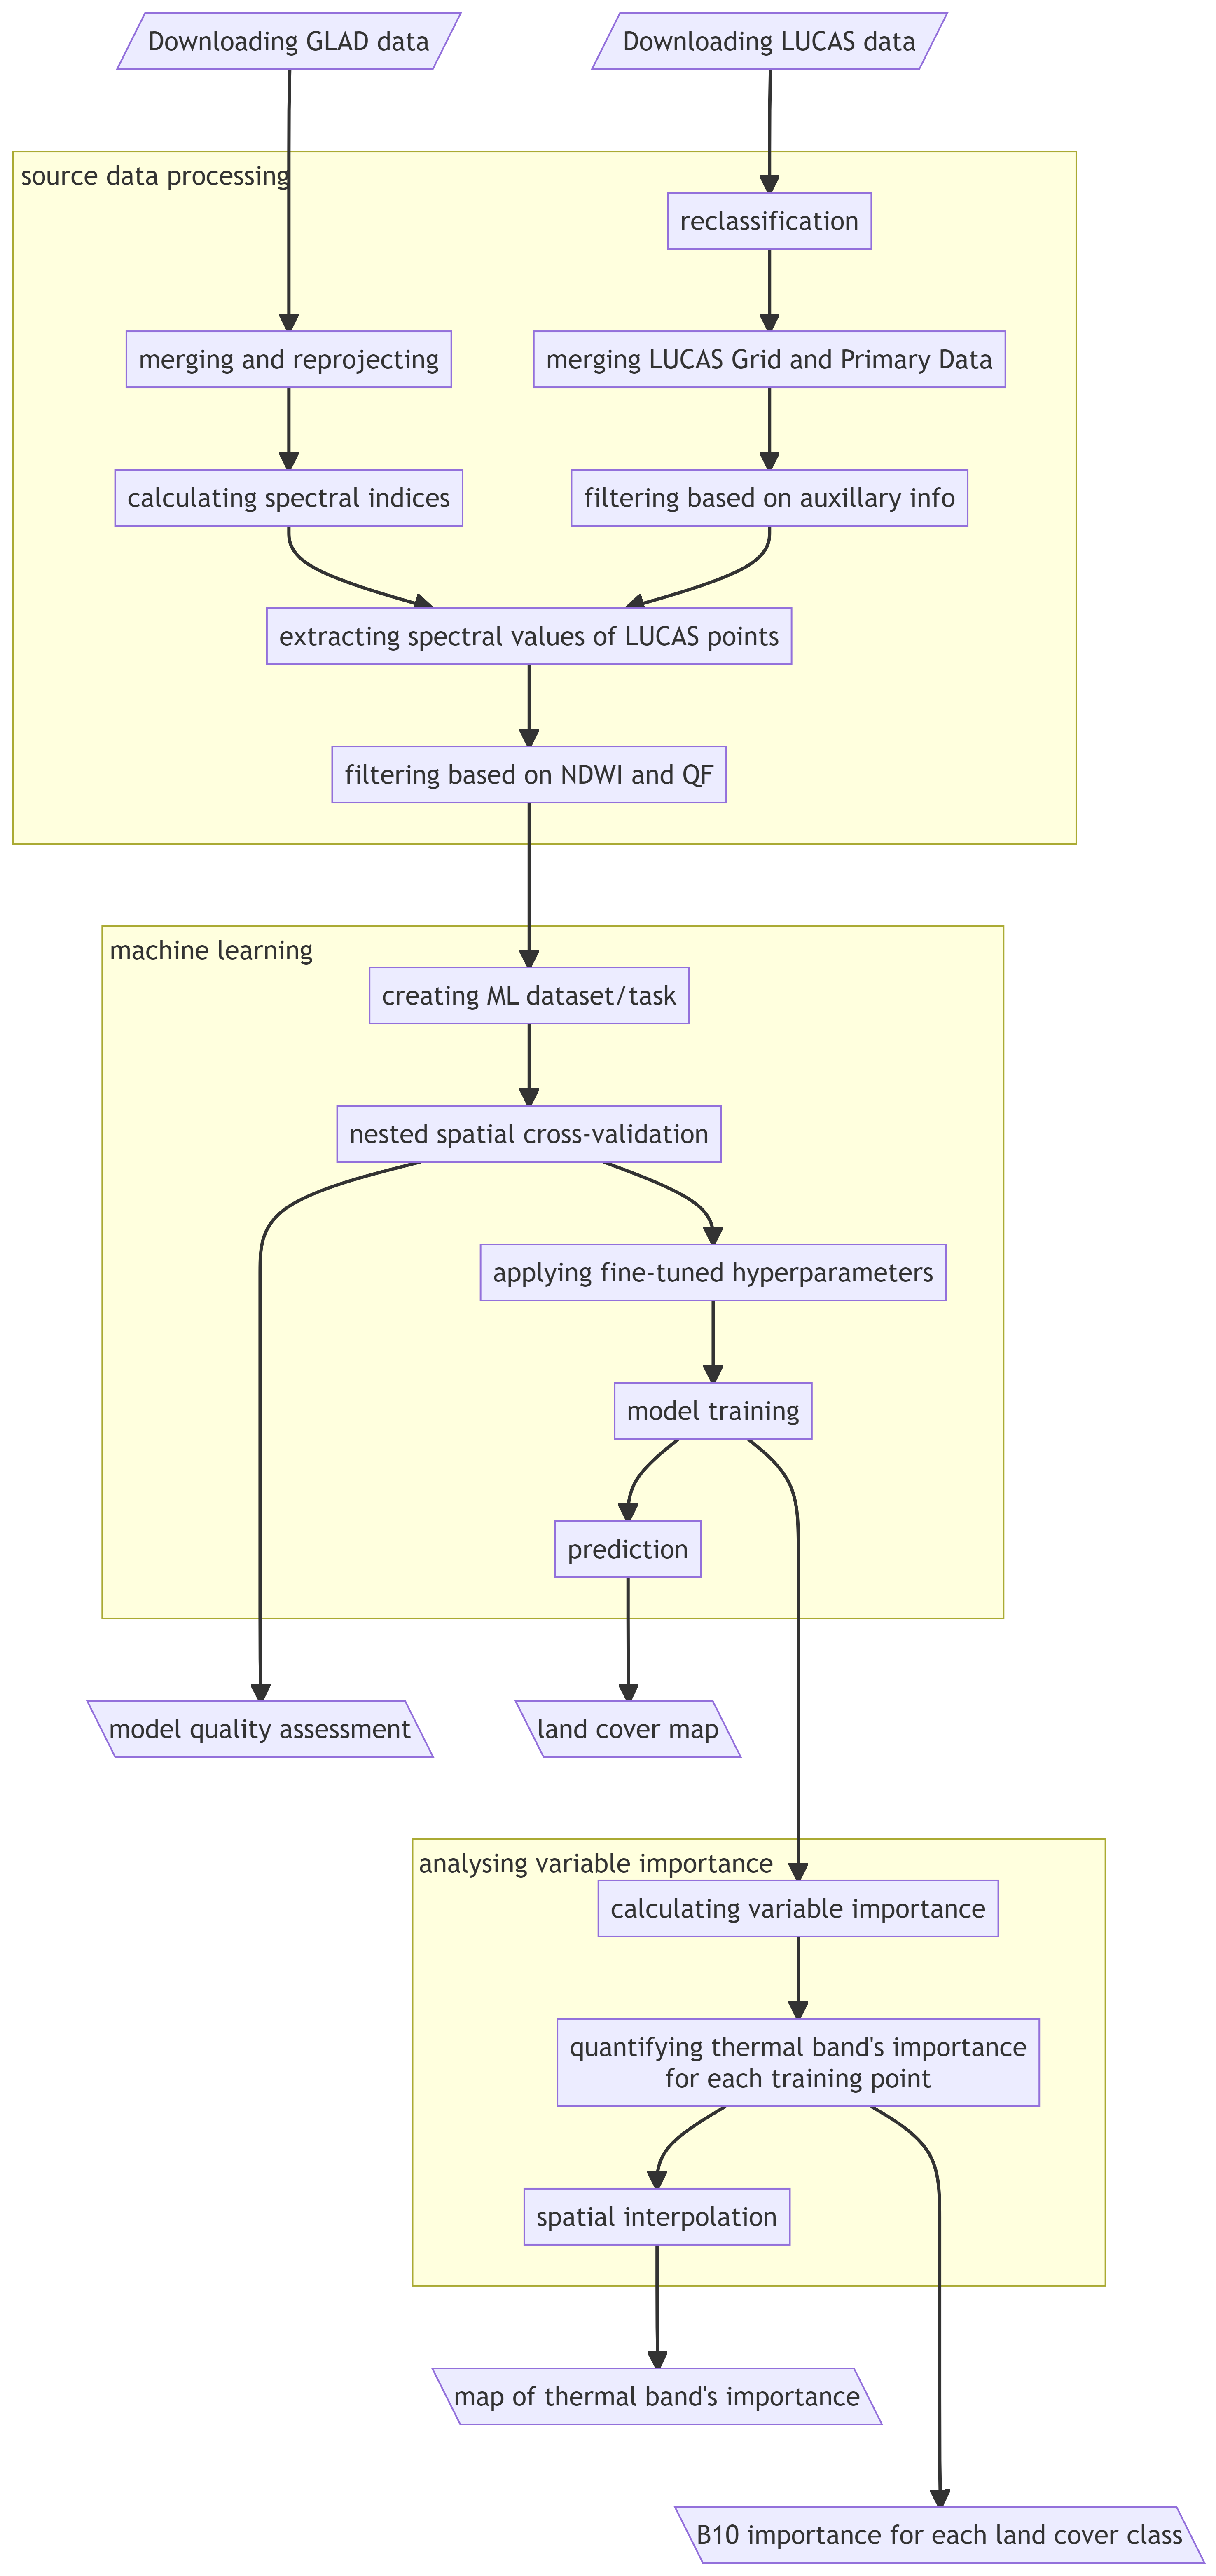
\includegraphics[width=4in,height=8.26in]{./02-roz2_files/figure-latex/mermaid-figure-1.png}

}

\end{figure}

}

\caption{\label{fig-rycina1}General workflow of the study}

\end{figure}

Landsat ARD dataset, provided by GLAD laboratory at the Univeristy of
Maryland, was used as a source of multi-spectral satellite imagery.
Training points were obtained from LUCAS dataset created by Eurostat
\autocite{dandrimont_harmonised_2020}. Both datasets were downloaded for
central-western part of Poland which was chosen as training area
(Figure~\ref{fig-rycina2}). This data was preprocessed and then used to
train the model and validate its performance.

\begin{figure}[t]

{\centering 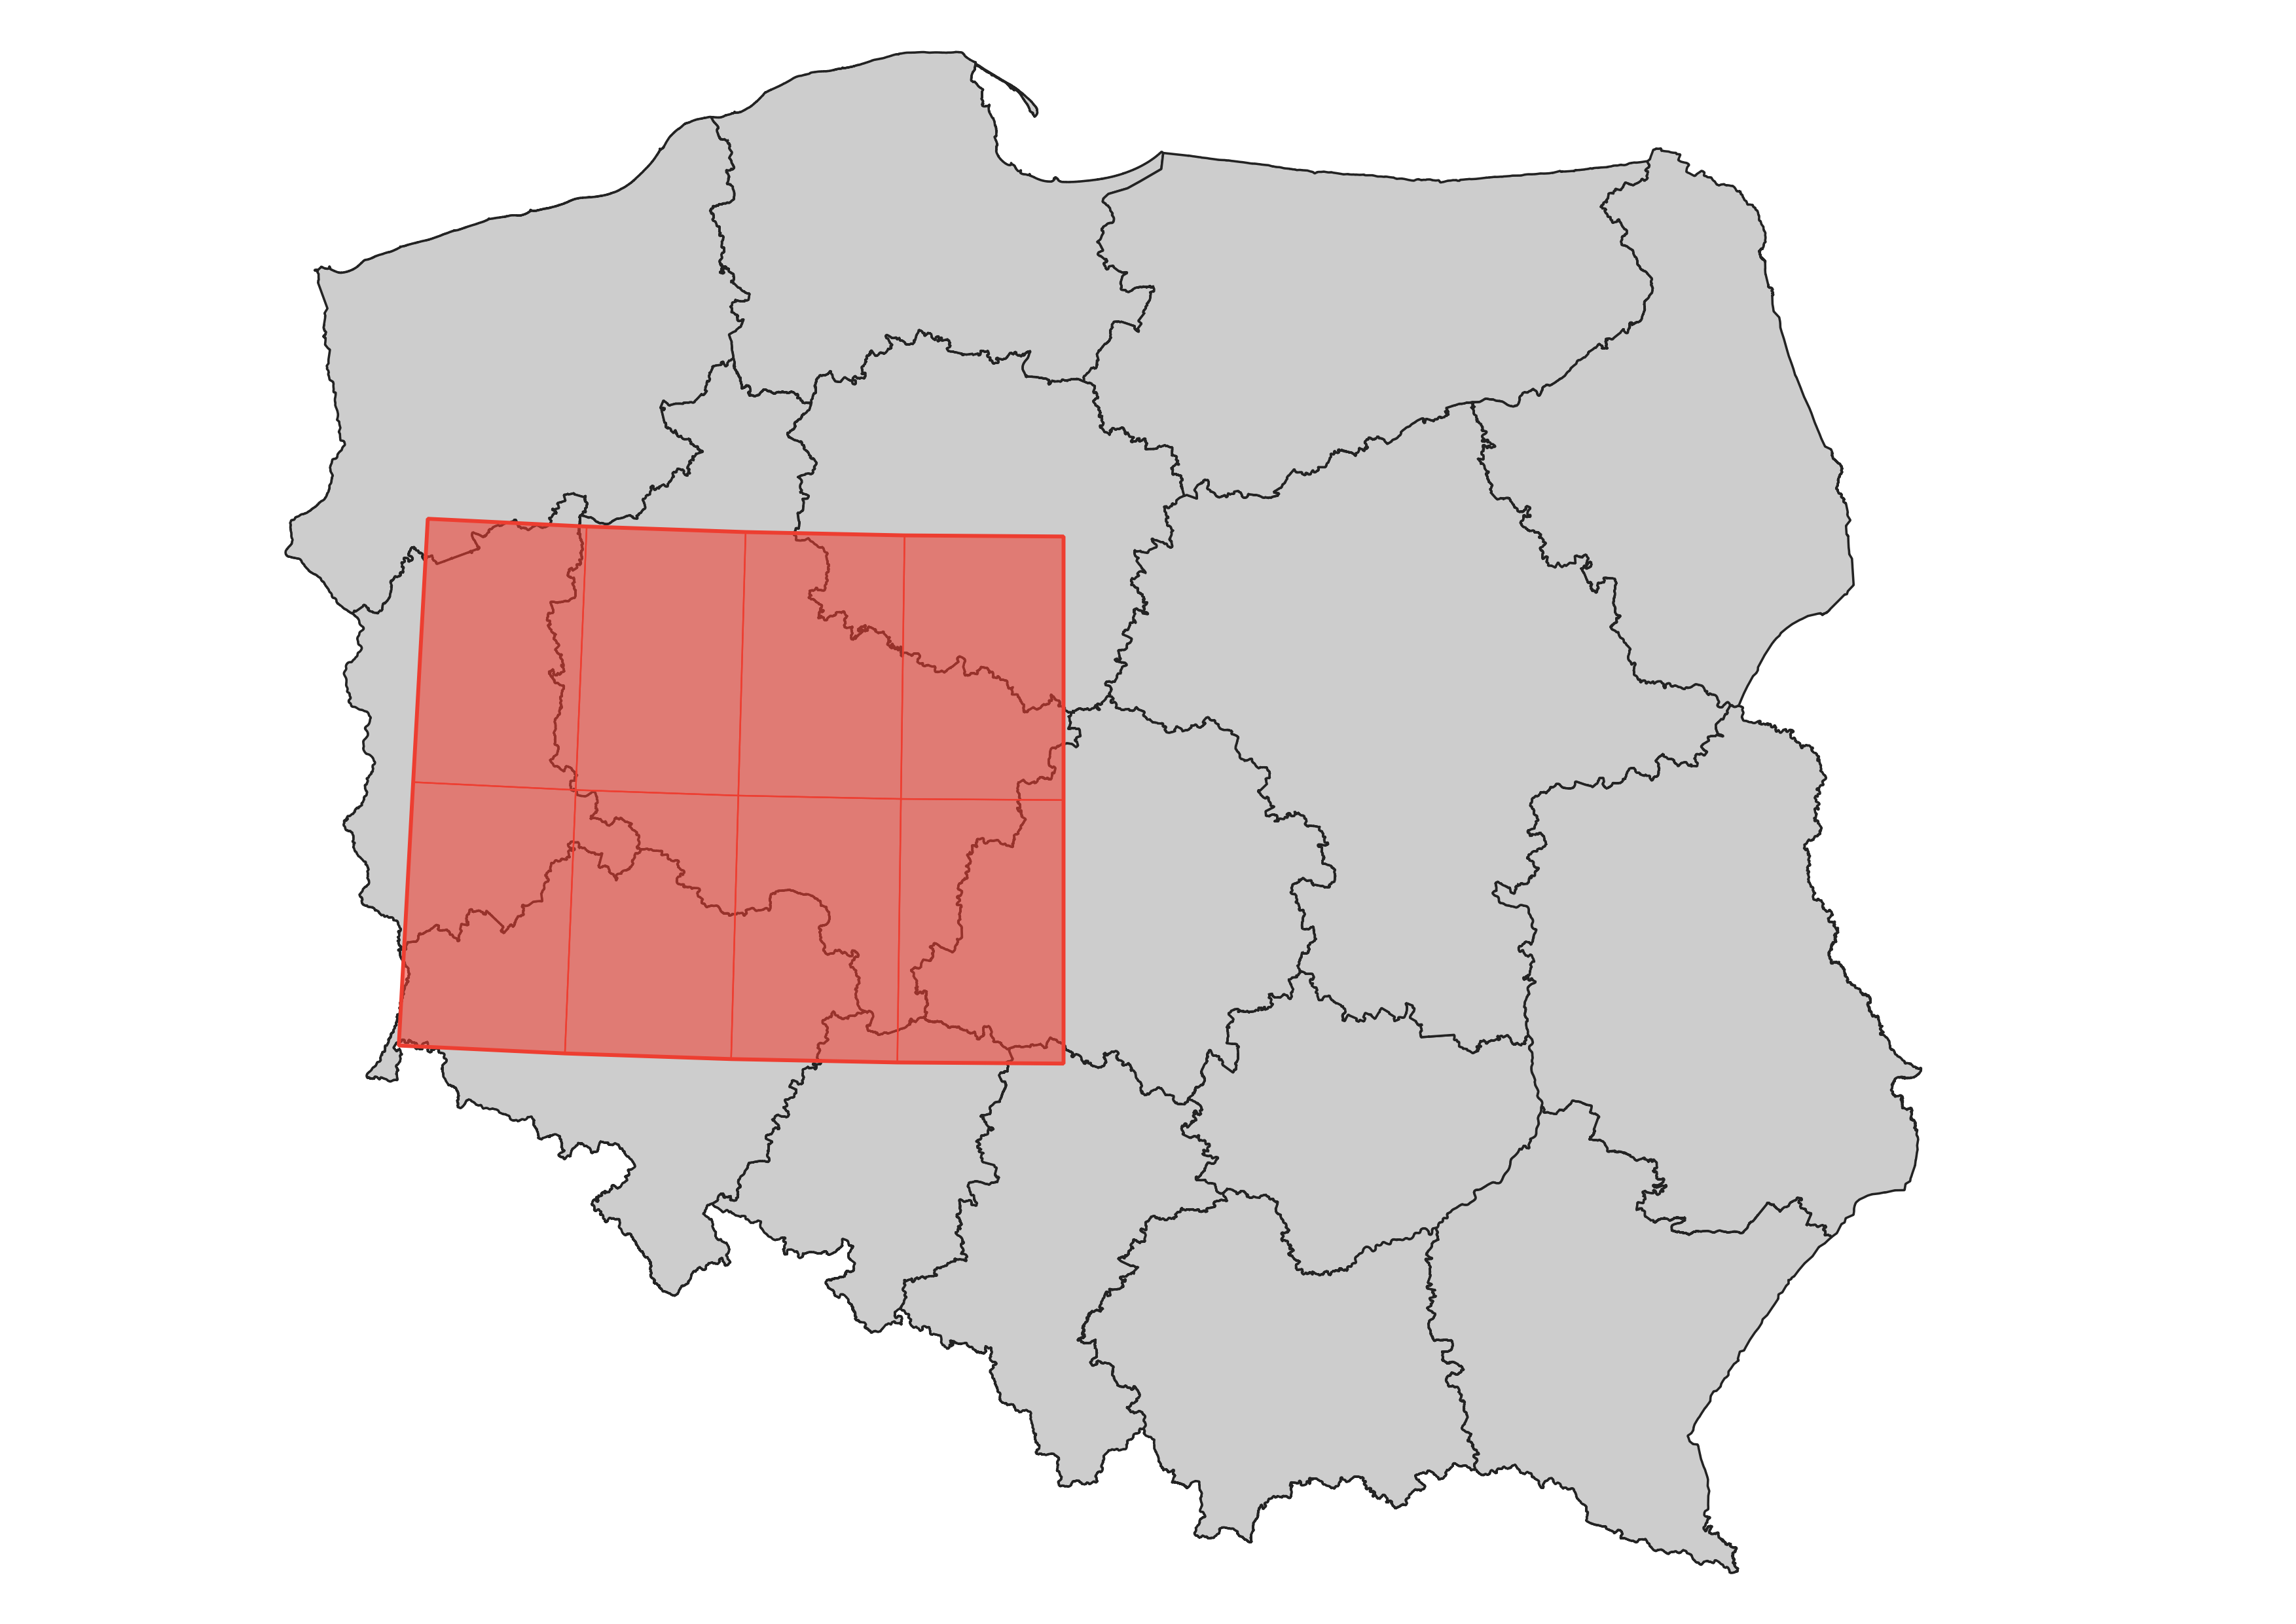
\includegraphics[width=5.875in,height=4.16667in]{./figures/study_area.png}

}

\caption{\label{fig-rycina2}Area covered by downloaded satellite
imagery}

\end{figure}

\hypertarget{sec-sat}{%
\section{Satellite imagery}\label{sec-sat}}

Satellite imagery from GLAD Landsat ARD product is available in 16-day
interval composites and is divided into 1° x 1° tiles. Processing of
original Landsat images performed by GLAD team included converting
spectral bands to top-of-atmosphere (TOA) reflectance, converting
thermal band to brightness temperature (BT) in Kelvins, scaling the
values of all bands, as well as, adding quality flag for every pixel
\autocite{potapov_landsat_2020}.

Satellite images for eight 1° x 1° tiles, covering the study area
(Figure \ref{fig-rycina1}), were downloaded using GLAD Tools v1.1 and
PERL programming language. These images are from 10th interval of the
year 2018, so downloaded mosaics consist of images created between
24.05.2018 and 8.06.2018. All downloaded images were merged and
reprojected from WGS84 coordinate reference system (EPSG:4326) to UTM
zone 33N (EPSG:32633). Every band was also resampled from its original
0.00025° resolution (corresponding to 27.83 m on the equator) to 30
meters.

In addition, four spectral indices were derived: Normalized Difference
Vegetation Index (NDVI), Modified Normalized Difference Water Index
(MNDWI), Normalized Difference Moisture Index (NDMI) and Modified Bare
soil Index (MBI). Formulas used to calculate these indices can be found
in Table~\ref{tbl-tabela1}.

\hypertarget{tbl-tabela1}{}
\begin{table}
\caption{\label{tbl-tabela1}Formulas of spectral indices dervied from Landsat data }\tabularnewline

\centering
\begin{tabular}{|>{\raggedright\arraybackslash}p{4cm}|>{}l|>{}l|}
\toprule
\textbf{band/index} & \textbf{abbreviation} & \textbf{formula}\\
\midrule
Blue & B2 & -\\
\hline
Green & B3 & -\\
\hline
Red & B4 & -\\
\hline
Near Infrared & B5 (NIR) & -\\
\hline
Short-wave Infrared 1 & B6 (SWIR1) & -\\
\hline
Short-wave Infrared 2 & B7 (SWIR2) & -\\
\hline
Thermal & B10 (TIRS1) & -\\
\hline
Normalized Difference Vegetation Index & NDVI & (B5 -B4) / (B4 + B5)\\
\hline
Modified Normalized Difference Water Index & MNDWI & (B3 - B6) / (B3 + B6)\\
\hline
Normalized Difference Moisture Index & NDMI & (B5 - B6) / (B5 + B6)\\
\hline
Modified Bare Surface Index & MBI & (B6 - B7 - B5) / (B6 + B7 + B5) + 0.5\\
\bottomrule
\end{tabular}
\end{table}

\hypertarget{sec-landcover}{%
\section{Land cover data}\label{sec-landcover}}

Data collected during LUCAS survey performed by Eurostat was chosen as
land cover training set. At the moment of writing, it is the most
accurate and comprehensive dataset containing information about land use
and land cover \autocite{pflugmacher_mapping_2019} due to the fact that
every point was either manually photo-interpreted or assessed during an
\emph{in-situ} visit.

LUCAS survey consists of two phases. The first phase is based on a grid
of points with 2km spacing covering whole territory of the European
Union (which equals to more than 1 million points). Each point of the
grid is visually interpreted using ortho-photos or satellite images, and
classified into one of seven major land-cover classes. These classes
are: arable land, permanent crops, grassland, wooded areas/shrub land,
bare land, artificial land and water. In the second phase, a subsample
of grid points is selected and then visited by Eurostat surveyors. They
classify each point according to full LUCAS land cover and land use
classification. The survey takes place in the spring and summer in order
to observe chosen places in their high vegetation season
\autocite{dandrimont_harmonised_2020}.

Surveyor not only assign land cover and land use classes to points, but
they also add auxillary information such as plant species present at the
site, percentage of land coverage of a chosen class, height of the trees
and their maturity, as well as information about local water management
and irrigation. If there are more than one land cover/land use types at
the point, observer can also assign a secondary class for every LUCAS
point.

Majority of the training points used in the classification model were
from the second phase of LUCAS survey, also called LUCAS Primary Data. I
downloaded a total of 4,153 points for the study area. Pre-processing
step included omitting records with missing data, excluding artificial
linear land cover classes (e.g.~roads or railways) and excluding points
that were surveyed more than 500 meters from their theoretical location.
In the next step, detailed land cover classes were aggregated into eight
main groups of land cover types. Two of them - grassland and shrubland
were additionally aggregated into one land cover class due to their
spectral and descriptive similarity. Then, I filtered some of the points
according to the percentage of land cover class coverage or percentage
of impervious surface coverage (Table~\ref{tbl-tabela2}). This step
reduced number of unreliable training points with mixed land cover,
e.g.~points with assigned class covering less than 50\% of surface
around it.

\hypertarget{tbl-tabela2}{}
\begin{table}
\caption{\label{tbl-tabela2}Filters applied to reclassified land cover groups. IMP - impervious
surface, HRB - herbaceous plants cover, TC - tree cover }\tabularnewline

\centering
\begin{tabular}{|>{}l|>{}l|>{}l|>{\raggedright\arraybackslash}p{4cm}|>{\raggedright\arraybackslash}p{2cm}|}
\toprule
\textbf{ID} & \textbf{LC class} & \textbf{LUCAS Grid} & \textbf{LUCAS Primary Data} & \textbf{Filters}\\
\midrule
\cellcolor[HTML]{e8ef5f}{\textbf{1}} & arable land & - & B00 (Cropland) & <30\% IMP\\
\hline
\cellcolor[HTML]{80dc59}{\textbf{2}} & grasslands & - & E00 (Grassland), D00 (Shrubland) & >50\% HRB; <30\% IMP\\
\hline
\cellcolor[HTML]{11a723}{\textbf{3}} & forests & - & C00 (Woodland) & >50\% TC; <20\% IMP\\
\hline
\cellcolor[HTML]{b7b7b7}{\textbf{4}} & bare land & 6 (Bare surface) & F00 (Bare land) & -\\
\hline
\cellcolor[HTML]{ea001f}{\textbf{5}} & artificial land & 7 (Artificial areas) & A00 (Artificial land) & >70\% IMP\\
\hline
\cellcolor[HTML]{56a4f3}{\textbf{6}} & water bodies & 8 (Inland water) & G00 (Water areas) & -\\
\hline
\cellcolor[HTML]{7a338c}{\textbf{7}} & wetlands & - & H00 (Wetlands) & -\\
\bottomrule
\end{tabular}
\end{table}

For the least frequent classes in the LUCAS Primary Data dataset - bare
land, artificial land and water bodies - I also added points classified
during the first phase of LUCAS survey (Figure~\ref{fig-rycina3}). This
step was necessary to ensure that every land cover class is represented
by enough number of points. It was not possible only for wetlands class,
because of lack of such category in the first phase classification. At
the end of the pre-processing, dataset had 3,778 training points
\autocite{oliver_buck_analysis_2015}.

\begin{figure}[t]

{\centering 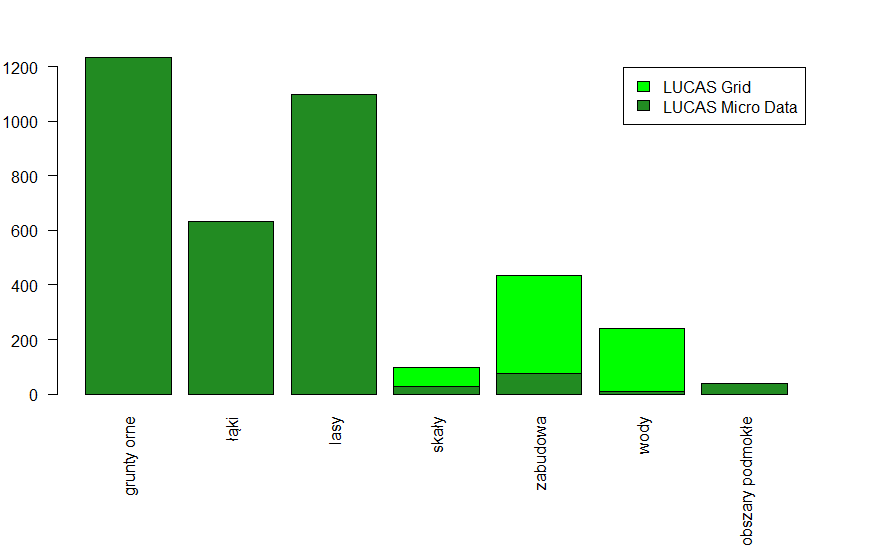
\includegraphics[width=5.75in,height=3.125in]{./figures/lucas_data.png}

}

\caption{\label{fig-rycina3}Distribution of points by land cover class
after pre-processing}

\end{figure}

After extracting values from Landsat ARD raster, LUCAS points were also
filtered using quality flag provided. Only points with clear-sky quality
flag were taken into account during the model training. Moreover, water
bodies points in which NDWI was lower than 0 were also excluded. These
two conditions eliminated over 400 points in total.

Training set obtained after pre-processing can be seen in
Figure~\ref{fig-rycina4}. Spatial distribution of data points was fairly
even and due to the structure of LUCAS data set, every point was located
2 kilometers or further from the next one.

\begin{figure}[t]

{\centering 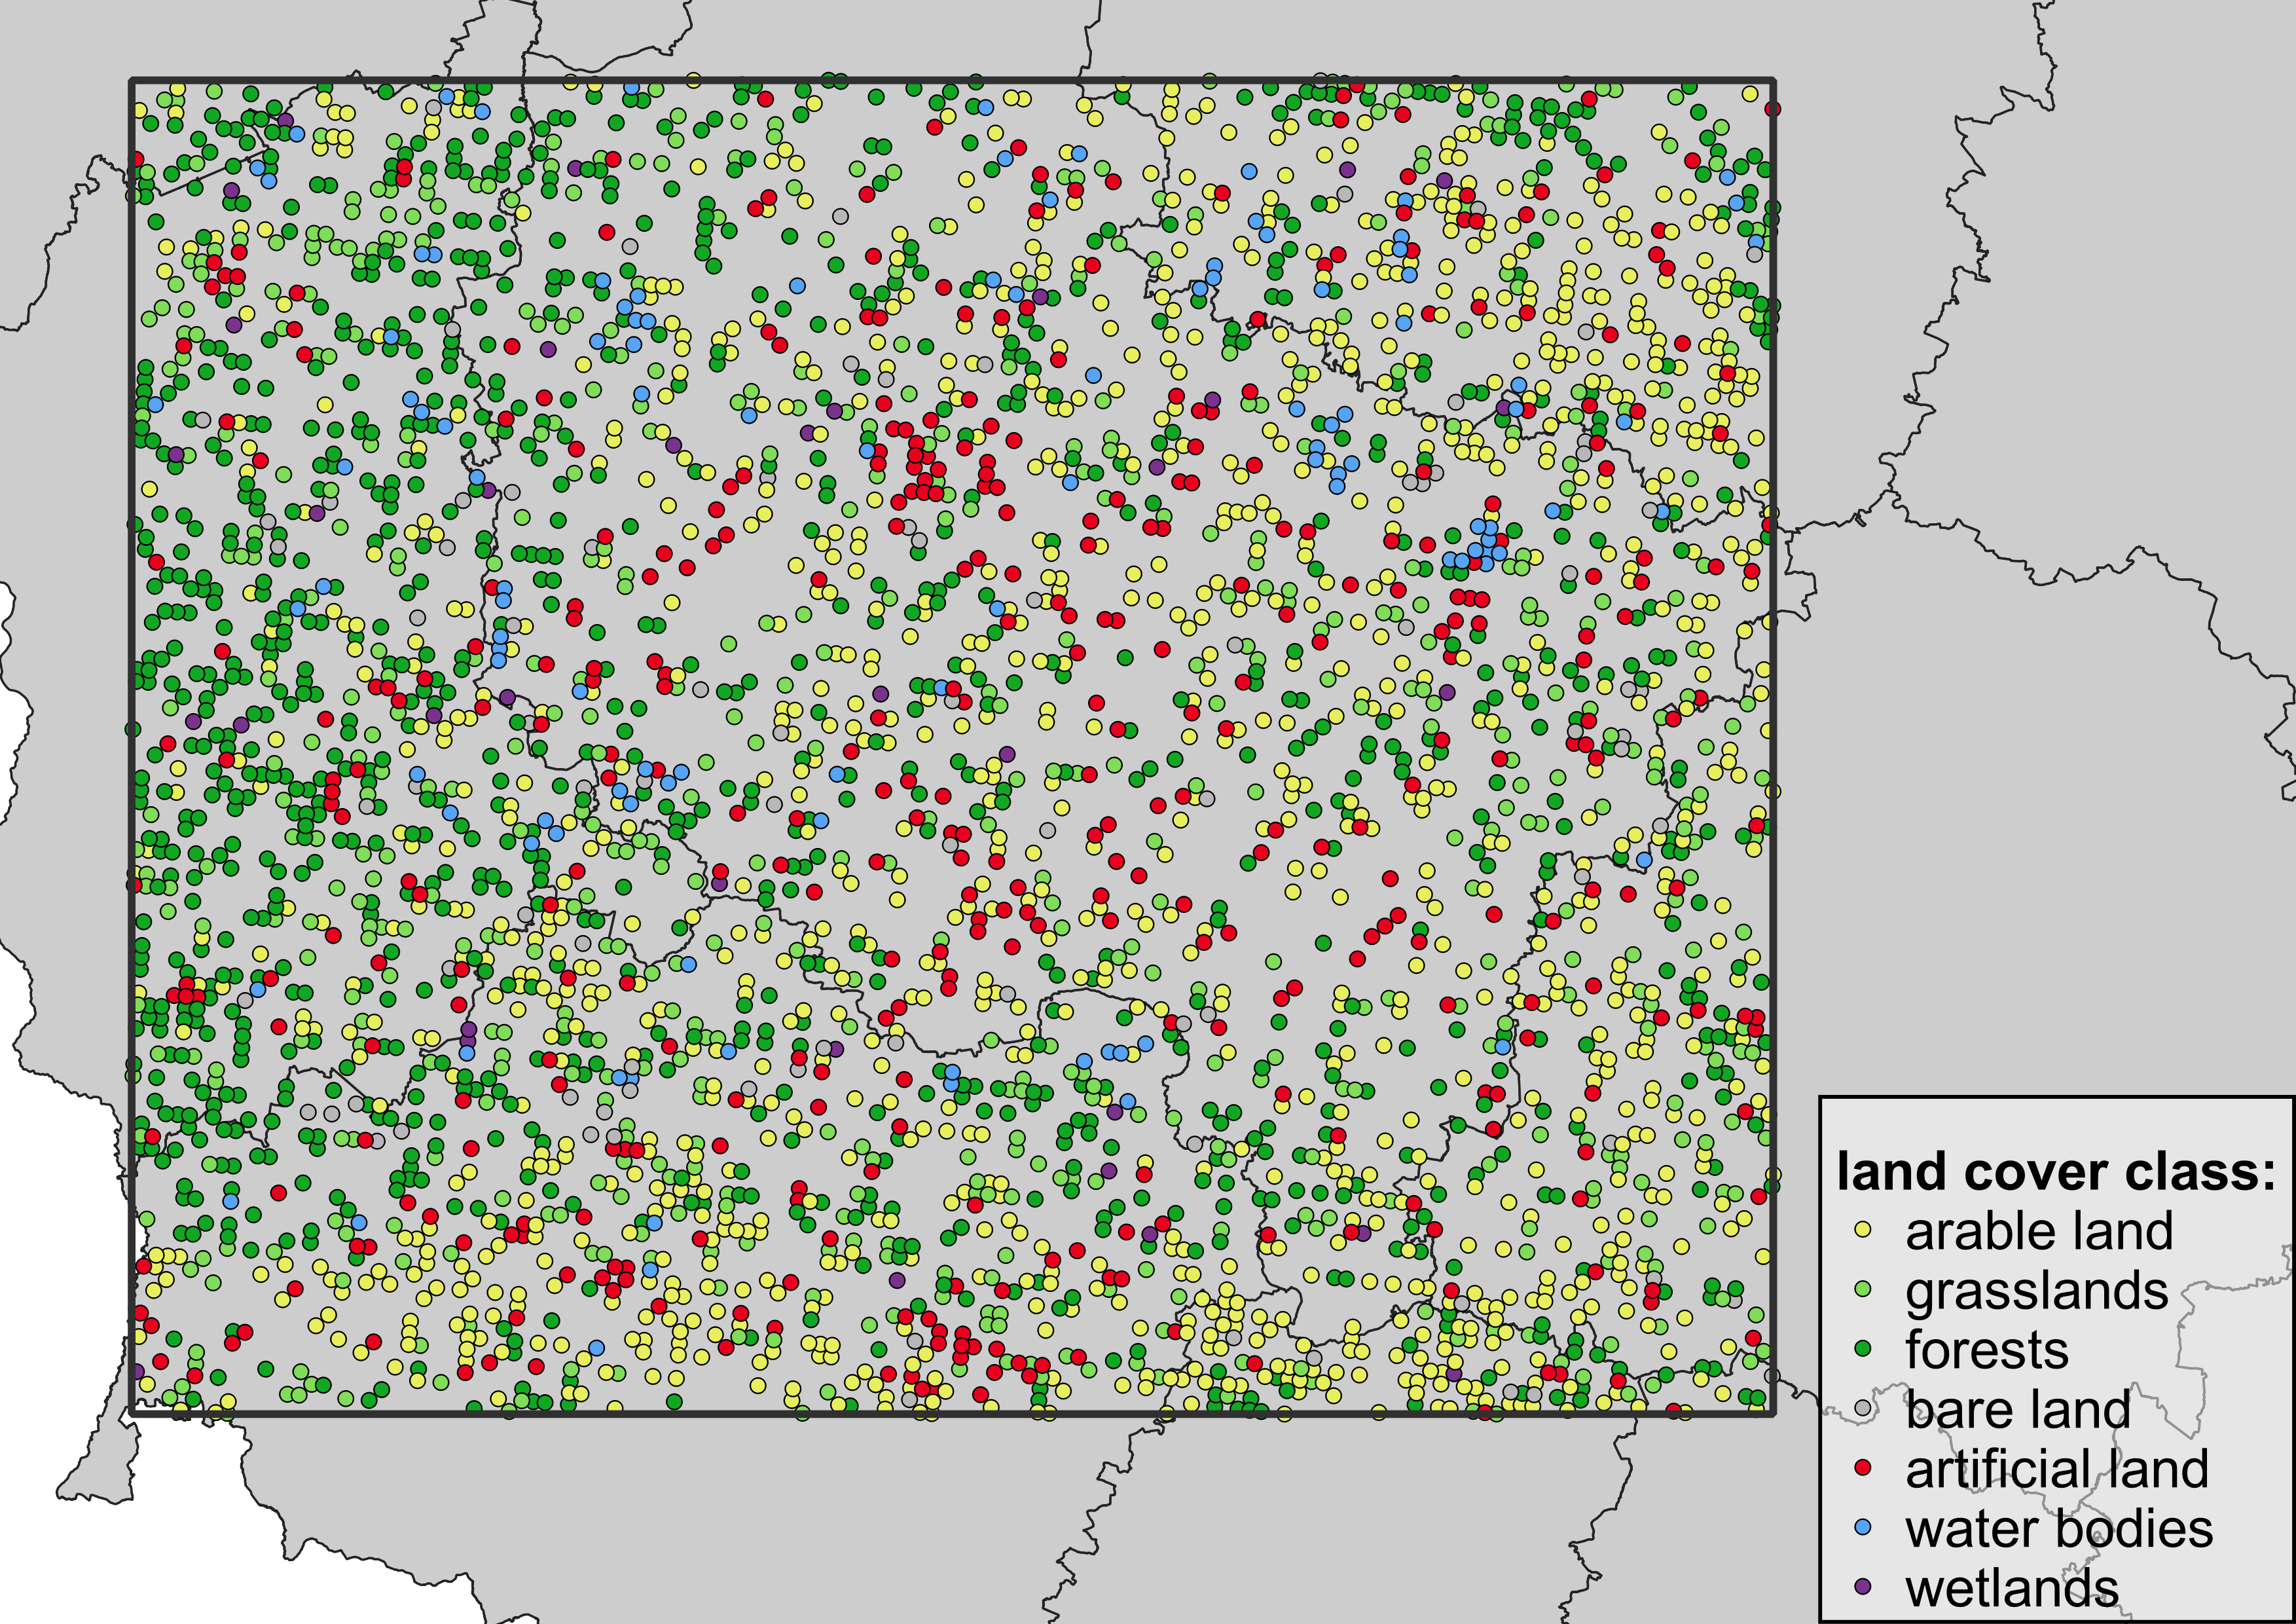
\includegraphics[width=5.875in,height=4.16667in]{./figures/lucas_distribution.png}

}

\caption{\label{fig-rycina4}Spatial distribution of LUCAS training
points after pre-processing}

\end{figure}

\hypertarget{sec-ml}{%
\section{Machine learning}\label{sec-ml}}

Machine learning is a computation method used to teach machines from
datasets automatically, without being specifically programmed
(\textcite{mahesh_machine_2018}; \textcite{sarker_machine_2021}). We can
divide machine learning methods into two main groups: supervised and
unsupervised.

Unsupervised learning analyzes unlabeled datasets without the need for
human intervention. This is widely used for extracting generative
features, identifying meaningful trends and structures, grouping results
and exploratory purposes \autocite{sarker_machine_2021}. This type of
machine learning discovers hidden patterns or data groupings (clusters)
which is used in exploration analysis or objects segmentation.

Supervised learning uses labeled training data and a collection of
training examples, which are used by an algorithm to find relationships
between different variables. It is carried out when certain goals are
identified to be accomplished from a certain set of inputs. There are
two main types of supervised learning tasks: classification (separating
data) and regression (fitting data) \autocite{sarker_machine_2021}.

In this study, supervised classification algorithm called Random Forest
(RF) was used \autocite{breiman_random_2001}.

\hypertarget{sec-rf}{%
\subsection{Random forest algorithm}\label{sec-rf}}

I chose Random Forest as an algorithm used in this study. It is a very
popular machine learning tool thanks to its high interpretability and
relatively high accuracy \autocite{qi_random_2012}. Other advantages of
this algorithm is its ability to handle missing values, wide spectrum of
accepted variable types (continuous, binary, categorical) and ease of
modelling high-dimensional data \autocite{qi_random_2012}. Random Forest
consists of a specified number of decision trees, which are based on
series of splitting rules.

Decision tree aims to partition the dataset into smaller, more
homogeneous groups \autocite{kuhn_applied_2013}. This process creates a
set of rules by dividing dataset into several categories. Each rule in
the decision tree is specified by a feature (variable used to split) and
a threshold (value of a feature dividing dataset)
\autocite{sekulic_random_2020}. Random forest algorithm is characterized
by using many decision trees at the same time and receiving results by
applying majority voting system based on outputs of all decision trees
\autocite{kuhn_applied_2013}. Each tree in the forest has slightly
different input data - a subset of data is sampled with replacement to
get different result in every tree. This process is known as bagging or
bootstrap aggregating \autocite{schonlau_random_2020}. Moreover,
algorithm is allowed to use only subset (randomly sampled) of available
variables which reduces correlation between trees
\autocite{sohil_introduction_2022}.

\hypertarget{sec-tuning}{%
\subsection{Parameter tuning}\label{sec-tuning}}

Random Forest algorithm takes several hyperparameters as an input in
order to specify how much should it fit to training data. Optimizing
these parameters is crucial for tree-based machine learning models
\autocite{yang_hyperparameter_2020}. Model's hyper-parameters can be
fine-tuned to find values that give the best model accuracy. I chose
three hyper-parameters for tuning: number of trees, maximum depth of the
forest and minimal size of each node in decision tree. Then, 10 models
with different hyper-parameter values chosen randomly from specified
search space were created and trained. I used overall accuracy achieved
by each classifier to rank their performance and choose parameters that
train the model the best. Parameters' search spaces and tuning results
can be found in Table~\ref{tbl-tabela3}.

\hypertarget{tbl-tabela3}{}
\begin{table}
\caption{\label{tbl-tabela3}Tuned parameters of RF model }\tabularnewline

\centering
\begin{tabular}{|>{}l|>{}l|>{}l|}
\toprule
\textbf{Hyper-parameter} & \textbf{Search space} & \textbf{Optimal value}\\
\midrule
number of trees & 50 - 400 & 272\\
\hline
maximum depth & 10 - 40 & 20\\
\hline
min. node size & 1 - 10 & 1\\
\bottomrule
\end{tabular}
\end{table}

\hypertarget{sec-resampling}{%
\subsection{Model quality assessment}\label{sec-resampling}}

Accuracy of the model was assessed using five performance measures:

\begin{itemize}
\item
  Overall accuracy: ratio of number of correct predictions to the total
  number of input points
\item
  Kappa coefficient: how well the classification performed as compared
  to randomly assigning values
\item
  Recall (producer's accuracy): how often are real features on the
  ground correctly shown on the classified map
\item
  Precision (user's accuracy): how often the class on the map will
  actually be present on the ground
\item
  F1-score: harmonic mean between precision and recall, measures if
  classifier both classifies data correctly and does not miss a
  significant number of points
\end{itemize}

Every above metric, except Kappa coefficient, take values from 0 to 1.
Value of 0 means poor model performance and value of 1 means high
quality of the model. As for Kappa coefficient, values range from -1 to
1. Values below 0 mean worse agreement between raters than random chance
and values above 0 (up to 1) mean model performing better than random.

Values of these indices were estimated with the help of resampling
technique called spatial cross-validation (CV). It is a type of
cross-validation that divides dataset into folds and also considers
spatial aspect of the data.

In \emph{k}-fold cross-validation, every data point is used in both
training and testing set. Whole dataset is randomly divided into
\emph{k} equal parts (\emph{folds}). Then, machine learning model is
independently trained \emph{k} times and in each run, different part of
the dataset is used as validation set while remaining \emph{k - 1} parts
are used to fit the model. This way, every data point is used in the
testing set only once and is used to train the model in the remaining
runs \autocite{jiao_performance_2016}. Usually, whole cross-validation
procedure is repeated several times to get higher number of unique
dataset splits and to receive more reliable average values of the
overall accuracy \autocite{varga_validation_2021}. Such approach is a
compromise which enables possibility of using a whole dataset in the
training process of the final model without a need of acquiring
independent testing set.

Since this study is based on geographic data, spatial autocorrelation
needs to be taken into account. As Tobler stated: ``Everything is
related to everything else, but near things are more related than
distant things'' \autocite{tobler_computer_1970}. In order to prevent
testing points from being related to training points, I applied spatial
cross-validation approach which aims to prevent the model to overfit to
the training data. This method is different than regular
cross-validation only in the partitioning step - instead of randomly
dividing dataset into groups, location of data points is used together
with k-means clustering \autocite{brenning_spatial_2012} in order to
create spatially disjoint folds \autocite{lovelace_geocomputation_2019}.
Thanks to this partitioning method, spatial bias can be significantly
reduced which leads to more reliable performance estimation. Example of
such approach can be seen on Figure~\ref{fig-rycina5}.

\begin{figure}[t]

{\centering 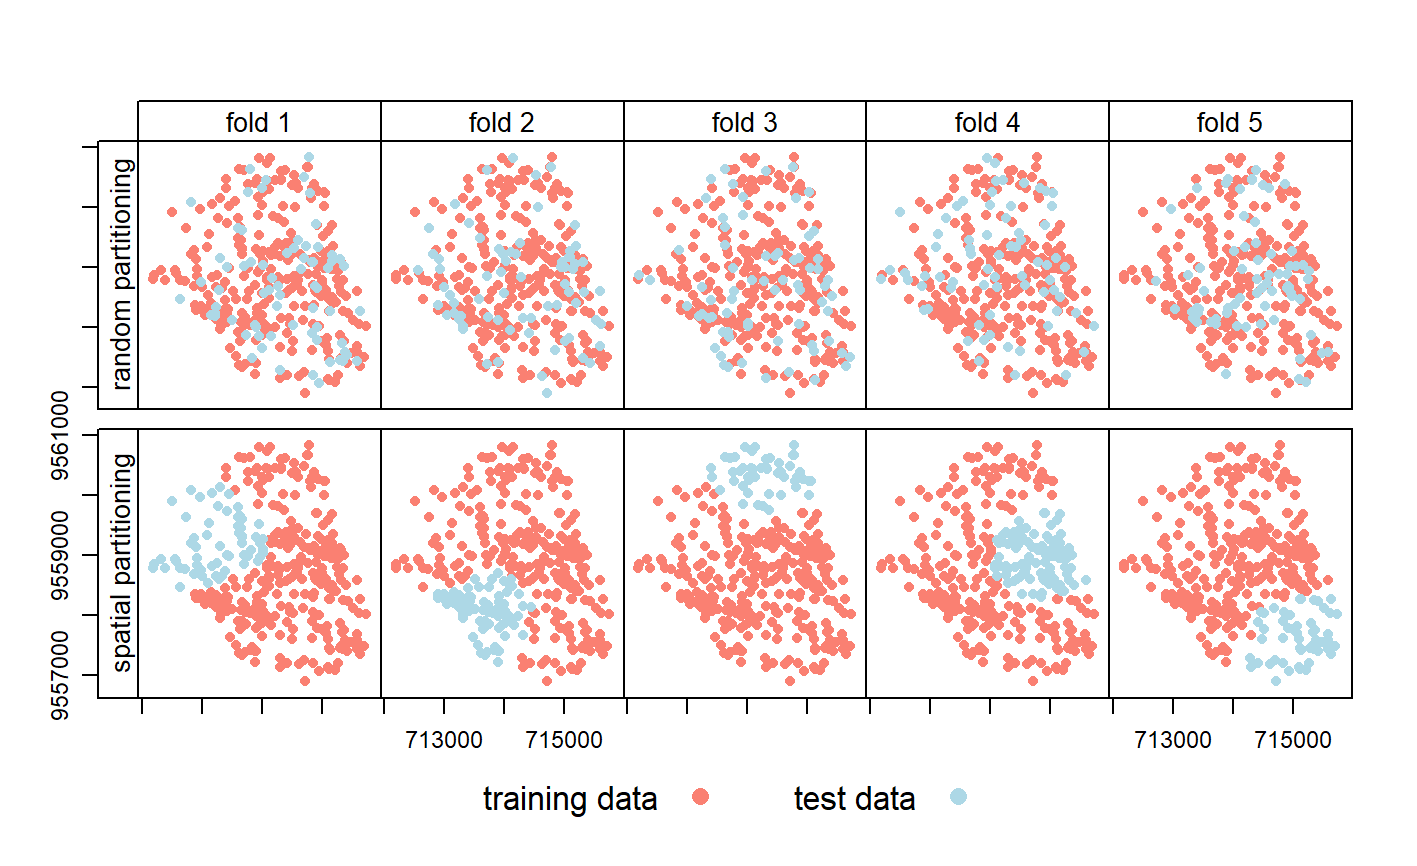
\includegraphics[width=5.9375in,height=3.64583in]{./figures/spatial_partitioning.png}

}

\caption{\label{fig-rycina5}Comparison of random and spatial
partitioning of dataset for cross-validation on external example data
(Source: \textcite{lovelace_geocomputation_2019})}

\end{figure}

With the aim to determine values of model's hyperparameters as
accurately as possible, I performed nested spatial cross-validation.
This method is an extension of previously described approach, with
hyperparameter tuning added to the process. Each fold created in the
spatial CV is further divided into next \emph{n} folds which comprise
the tuning level of the process. Then, another cross-validation is
performed on these folds in order to determine performance of randomly
sampled hyperparameter values. The best hyperparameter combination is
chosen to train the model on outer fold on performance estimation level
\autocite{schratz_hyperparameter_2019}. Whole process is then repeated
on every of \emph{k} outer folds which leads to most accurate
performance measurement as well as defining the best hyperparameter
setting. FIGURE?

\hypertarget{sec-importance}{%
\section{Variable importance and its spatial
distribution}\label{sec-importance}}

Quantifying importance of model's variables is a part of evaluating its
results. It can be used for model simplification and exploration,
domain-knowledge-based validation or knowledge generation
\autocite{biecek_explanatory_2021}. This study was focused on the latter
purpose since its aim was to check if thermal information has an impact
on land-cover classification.

Importance of model variables can be measured on two levels: dataset
level and instance level \autocite{biecek_explanatory_2021}. On the
dataset level, we can measure change in model's accuracy depending on
the presence of one chosen variable
(Section~\ref{sec-importance-dataset}). This gives basic knowledge about
this variable's impact on model predictions. Assessing importance on the
instance level helps to understand an impact of variables for one
specific data point (Section~\ref{sec-importance-instance}). Moreover,
the instance level importance can be utilized to interpolate variable
importance values from points into continuous raster data
(Section~\ref{sec-importance-distribution}).

\hypertarget{sec-importance-dataset}{%
\subsection{Dataset level}\label{sec-importance-dataset}}

Measuring variable importance on the dataset level requires evaluating
model twice: once with original data and once with permuted values of
the considered variable. The main idea behind this action is to measure
difference between models' performance. Breiman
\autocite*{breiman_random_2001} assumes that if a variable is important,
then it is expected to lower model's performance after permuting its
values. For this purpose, cross entropy was used as a loss function thus
its change was considered as a measure of variable importance
\autocite{biecek_explanatory_2021}. In order to measure each variable's
importance, twelve seperate models were created: one with original data
and eleven modified models, each one with different variable's values
permuted. Comparison of these eleven models and original model made
possible quantifying impact of every variable on original model's
results. This value is treated as overall variable importance on the
dataset level.

There is also more visual method to explore variable importance on
dataset level. It is based on interpreting partial-dependence (PD)
profiles of variables (Figure~\ref{fig-rycina6}). Such type of plot
shows how does probability of choosing certain class changes as a
function of the selected variable \autocite{biecek_explanatory_2021}.
Values for PD profile are calculated by averaging Ceteris-paribus
profiles created for every observation in the dataset. This approach is
an easy and intuitive way to understand variables' impact on model
results. If probability values of choosing certain class do not change
along with changes of variable's value, we can assume that this variable
does not have big impact on model predictions or that our model did not
detect such dependence.

\begin{figure}[t]

{\centering 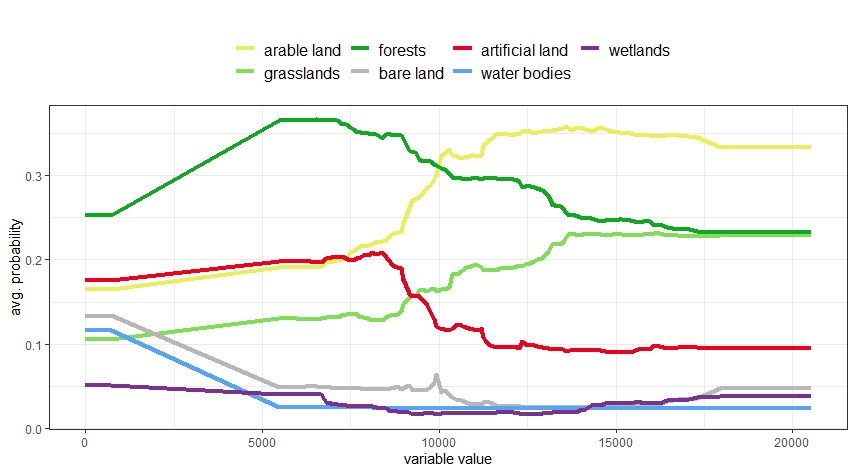
\includegraphics[width=5.90625in,height=3.125in]{./figures/profB5.png}

}

\caption{\label{fig-rycina6}Example variable profile for near-infrared
band (B5).}

\end{figure}

\hypertarget{sec-importance-instance}{%
\subsection{Instance level}\label{sec-importance-instance}}

Another way to measure variable importance in machine learning models is
the instance level evaluation. It helps to find out how much each
variable contributed to the classification result for a particular
observation \autocite{biecek_explanatory_2021}. One way of calculating
variable impact on the observation result is creating break-down plot
(Figure~\ref{fig-rycina7}). Its main idea is to estimate contribution of
variable by measuring the change in model's predictions while fixing the
values of consecutive variables to values recorded for the chosen
observation \autocite{biecek_explanatory_2021}. After fixing the value
of variable for whole dataset, change in model's prediction is
calculated. This value indicates variable impact on a chosen
observation.

\begin{figure}[t]

{\centering 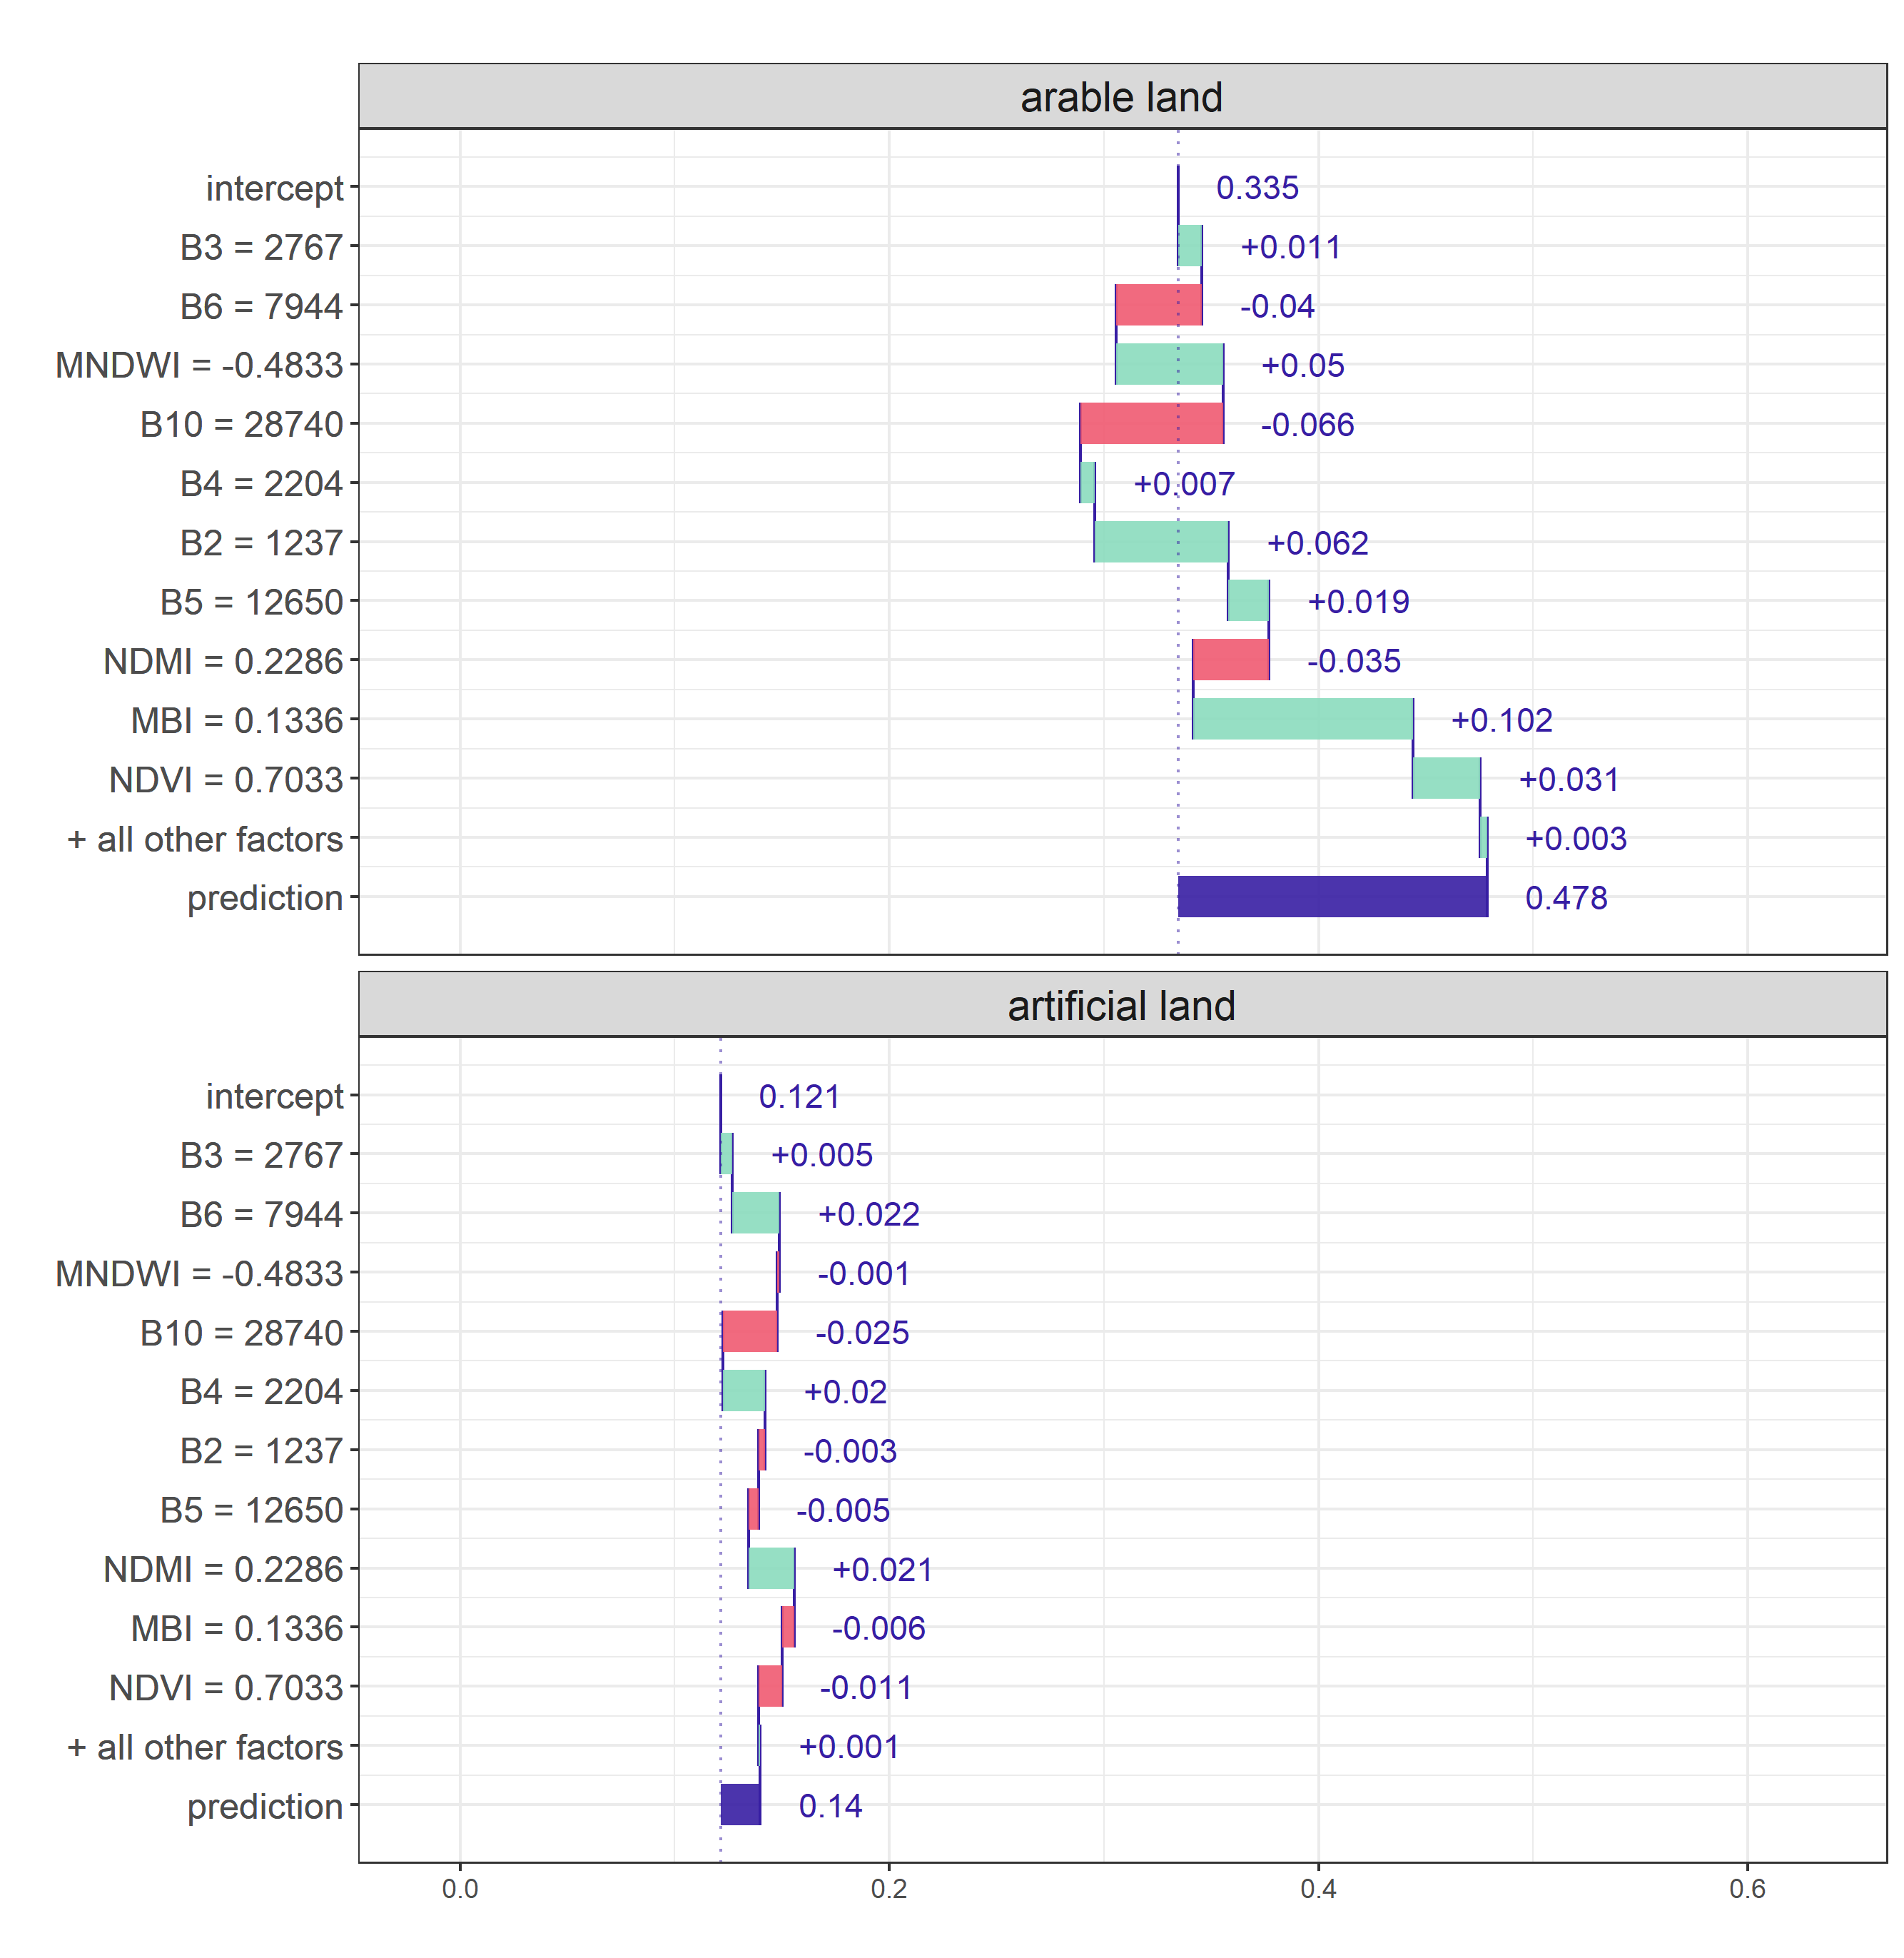
\includegraphics[width=0.7\textwidth,height=5.20833in]{./figures/break-down_plot.png}

}

\caption{\label{fig-rycina7}Example of a break-down plot that visualises
variables' impact on chosen observation}

\end{figure}

However, above method is highly dependent on variable ordering and
interactions between these variables \autocite{biecek_explanatory_2021}.
To address this issue, I applied another approach based on averaging
values from multiple break-down plots, each one with different ordering
of the variables. This method originates from ``Shapley values''
\autocite{shapley_value_1953} and was adapted to machine learning by
Štrumbelj and Kononenko \autocite*{strumbelj_efficient_2010}. Main idea
of this approach is to apply several different variable orderings,
create a break-down plot for each of them and calculate the mean value
of contribution for each variable (Figure~\ref{fig-rycina8}). Thanks to
this method, the influence of variable ordering can be mostly removed
\autocite{biecek_explanatory_2021}.

\begin{figure}[t]

{\centering 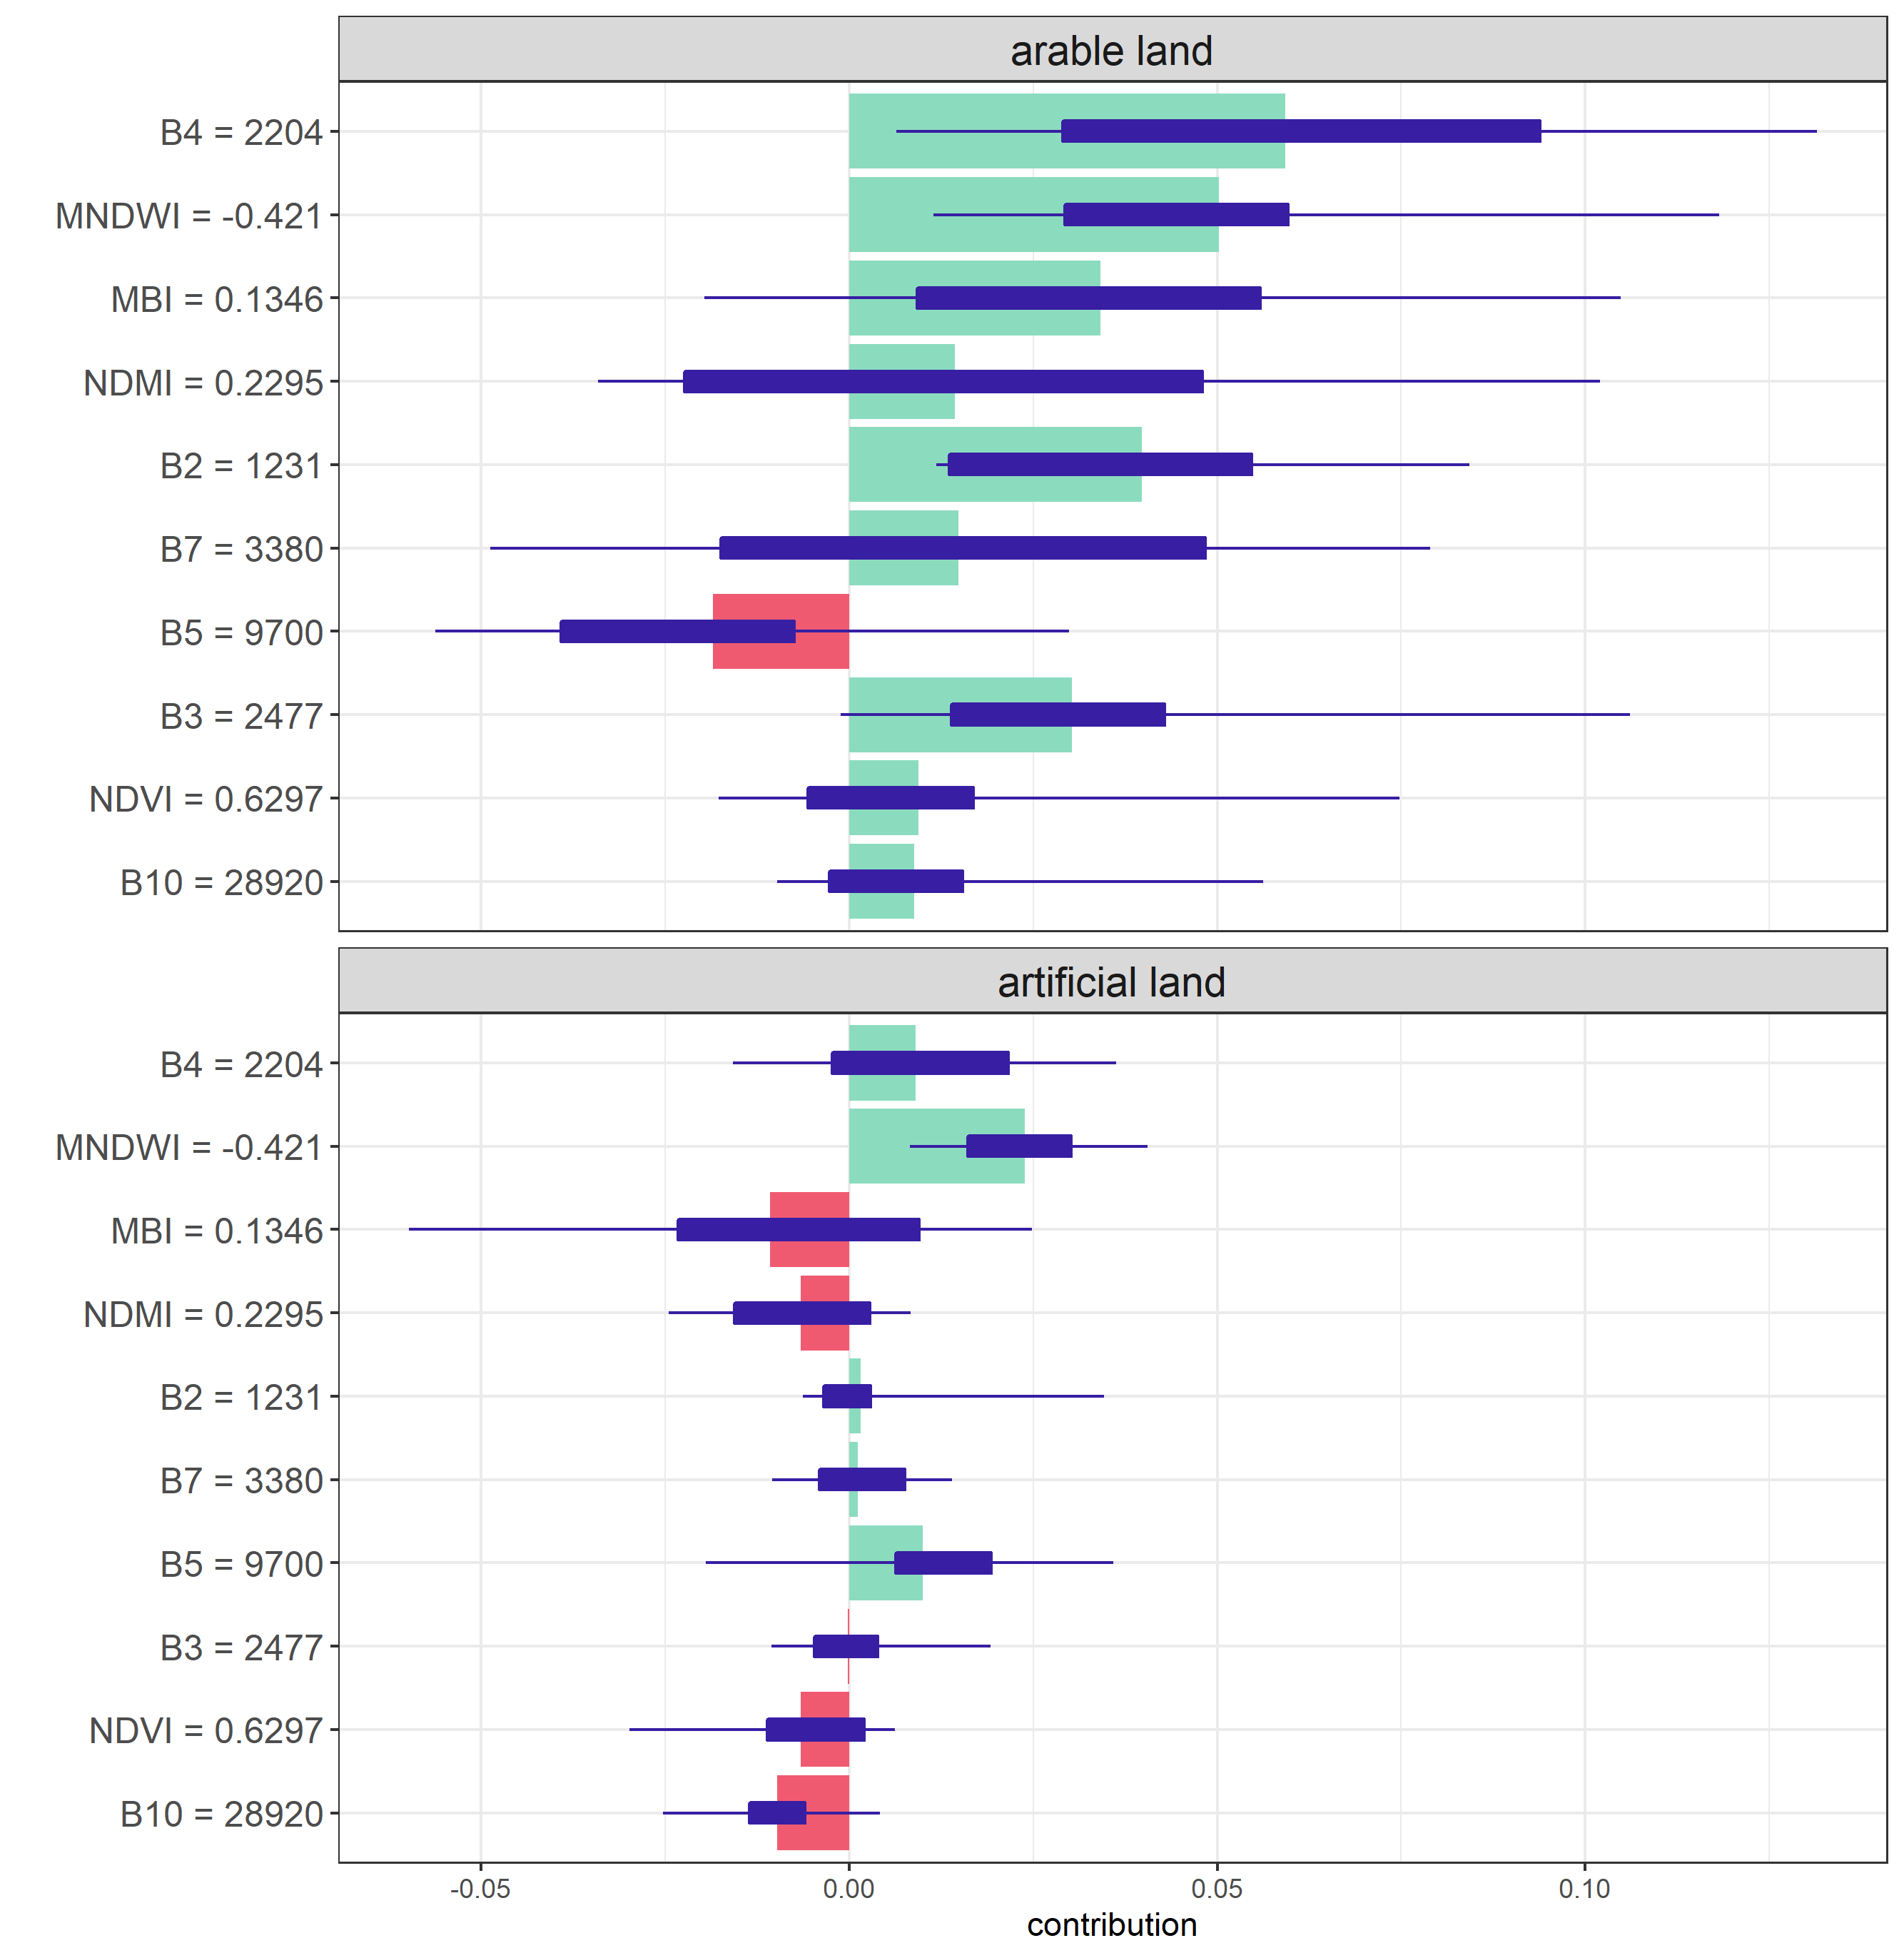
\includegraphics[width=0.7\textwidth,height=5.20833in]{./figures/shapley_values.png}

}

\caption{\label{fig-rycina8}Example plot of Shapley Additive
Explanations}

\end{figure}

Eventually, Shapley values provide a possibilty to measure contribution
of each variable in every observation in the training set. Such result
enables us to add spatial context to the variable importance, which is
further described in Section \ref{sec-importance-distribution}.

\hypertarget{sec-importance-distribution}{%
\subsection{Spatial distribution}\label{sec-importance-distribution}}

In order to estimate spatial distribution of variable importance values,
I applied two different approaches. First of them is based on the raster
aggregation - resampling of satellite imagery from 30 m to 1.5 km
resolution. Lowering the resolution of the data and averaging bands'
values highly decreases computational time, as well as helps to discover
more general trends and patterns rather than local ones. After
resampling, Shapley values are calculated for every raster cell and
variable importance value is quantified.

The second approach utilizes LUCAS training points used during a model
training together with spatial interpolation techniques. First, Shapley
values are calculated for every point and importance of variable is
assigned to them. This step is followed by spatial interpolation of
variable importance values from points to continuous raster layer with
the help of the Inverse Distance Weighting (IDW) interpolation method.

Both approaches have their pros and cons. Raster aggregation method is
spatially more consistent, but averaging of spectral values may not
entirely represent objects on the ground. On the other hand, point
interpolation method is very accurate for places near LUCAS points
location, but values for more distant objects may not be as reliable.

\hypertarget{sec-r}{%
\section{R language environment}\label{sec-r}}

Almost every step of analysis described in previous sections was
performed with use of R \autocite{R-base} - an open-source programming
language designed mainly for statistical computing and visualizing data.
I used RStudio \autocite{rstudio_team_rstudio_2020} as an integrated
development environment (IDE). Apart from base R functionalities, a
number of packages created by the R community were implemented into
workflow. I used \emph{terra} package \autocite{R-terra} to perform
raster data operations and \emph{sf} \autocite{R-sf} to manipulate and
process vector data. To conduct machine learning steps of the analysis,
I used an environment of various machine learning packages called
\emph{mlr3} \autocite{R-mlr3}. Random forest algorithm used by
\emph{mlr3} framework is part of the \emph{ranger} package
\autocite{R-ranger}. I also used \emph{dplyr} \autocite{R-dplyr} and
\emph{tidyr} packages \autocite{R-tidyr} to clean and process tabular
data. \emph{DALEX} \autocite{R-DALEX} and \emph{DALEXtra}
\autocite{R-DALEXtra} packages provided various functionalities enabling
me to estimate variable importance and visualize these results with the
help of \emph{ggplot2} package \autocite{R-ggplot2}. Package called
\emph{gstat} \autocite{R-gstat} helped to interpolate variable
importance values from points to a continuous raster layer. In addition,
\emph{future} package \autocite{R-future} was used to enable
multi-threading of some computationally intensive tasks.

\bookmarksetup{startatroot}

\hypertarget{sec-results-map}{%
\chapter{Result of the model - land cover map}\label{sec-results-map}}

\begin{itemize}
\tightlist
\item
  land cover map of Poznań metropolitan area
\end{itemize}

\begin{figure}[t]

{\centering 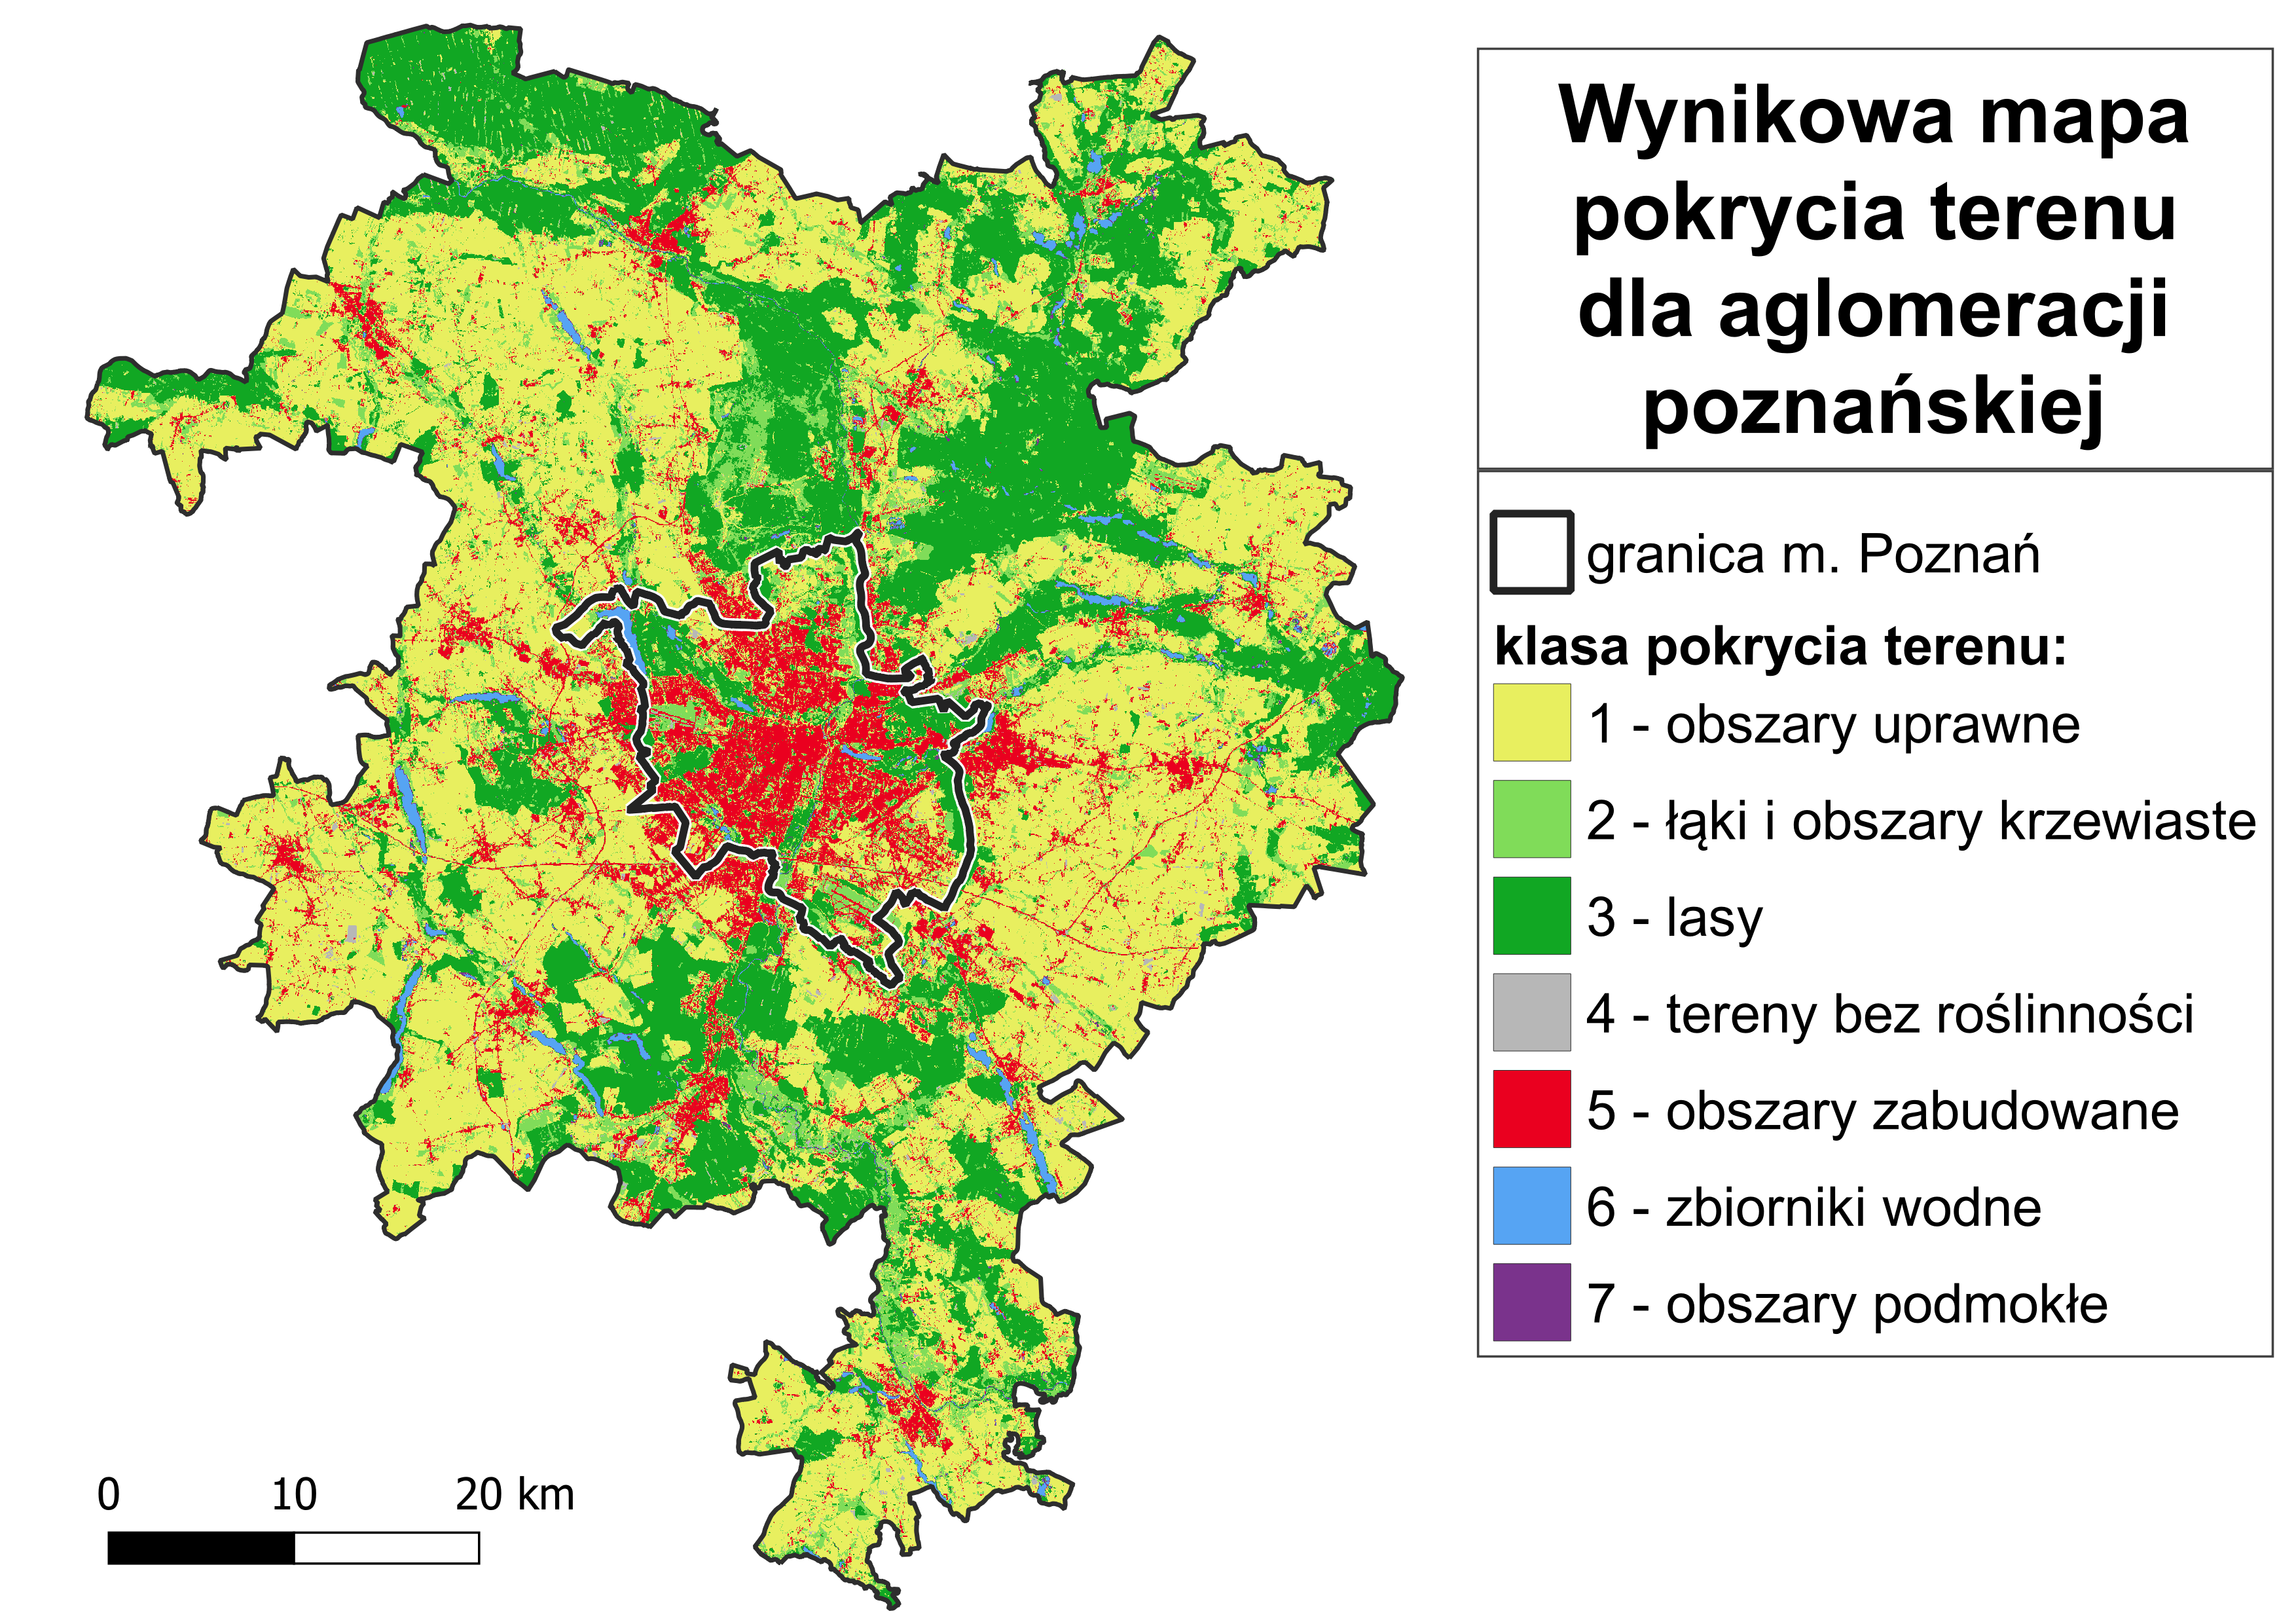
\includegraphics[width=5.875in,height=4.16667in]{./figures/result_map.png}

}

\caption{\label{fig-rycina9}Land cover map of Poznań metropolitan area
created during this study.}

\end{figure}

\begin{itemize}
\tightlist
\item
  comparison of land cover map and RGB satellite imagery
\end{itemize}

\begin{figure}[t]

{\centering 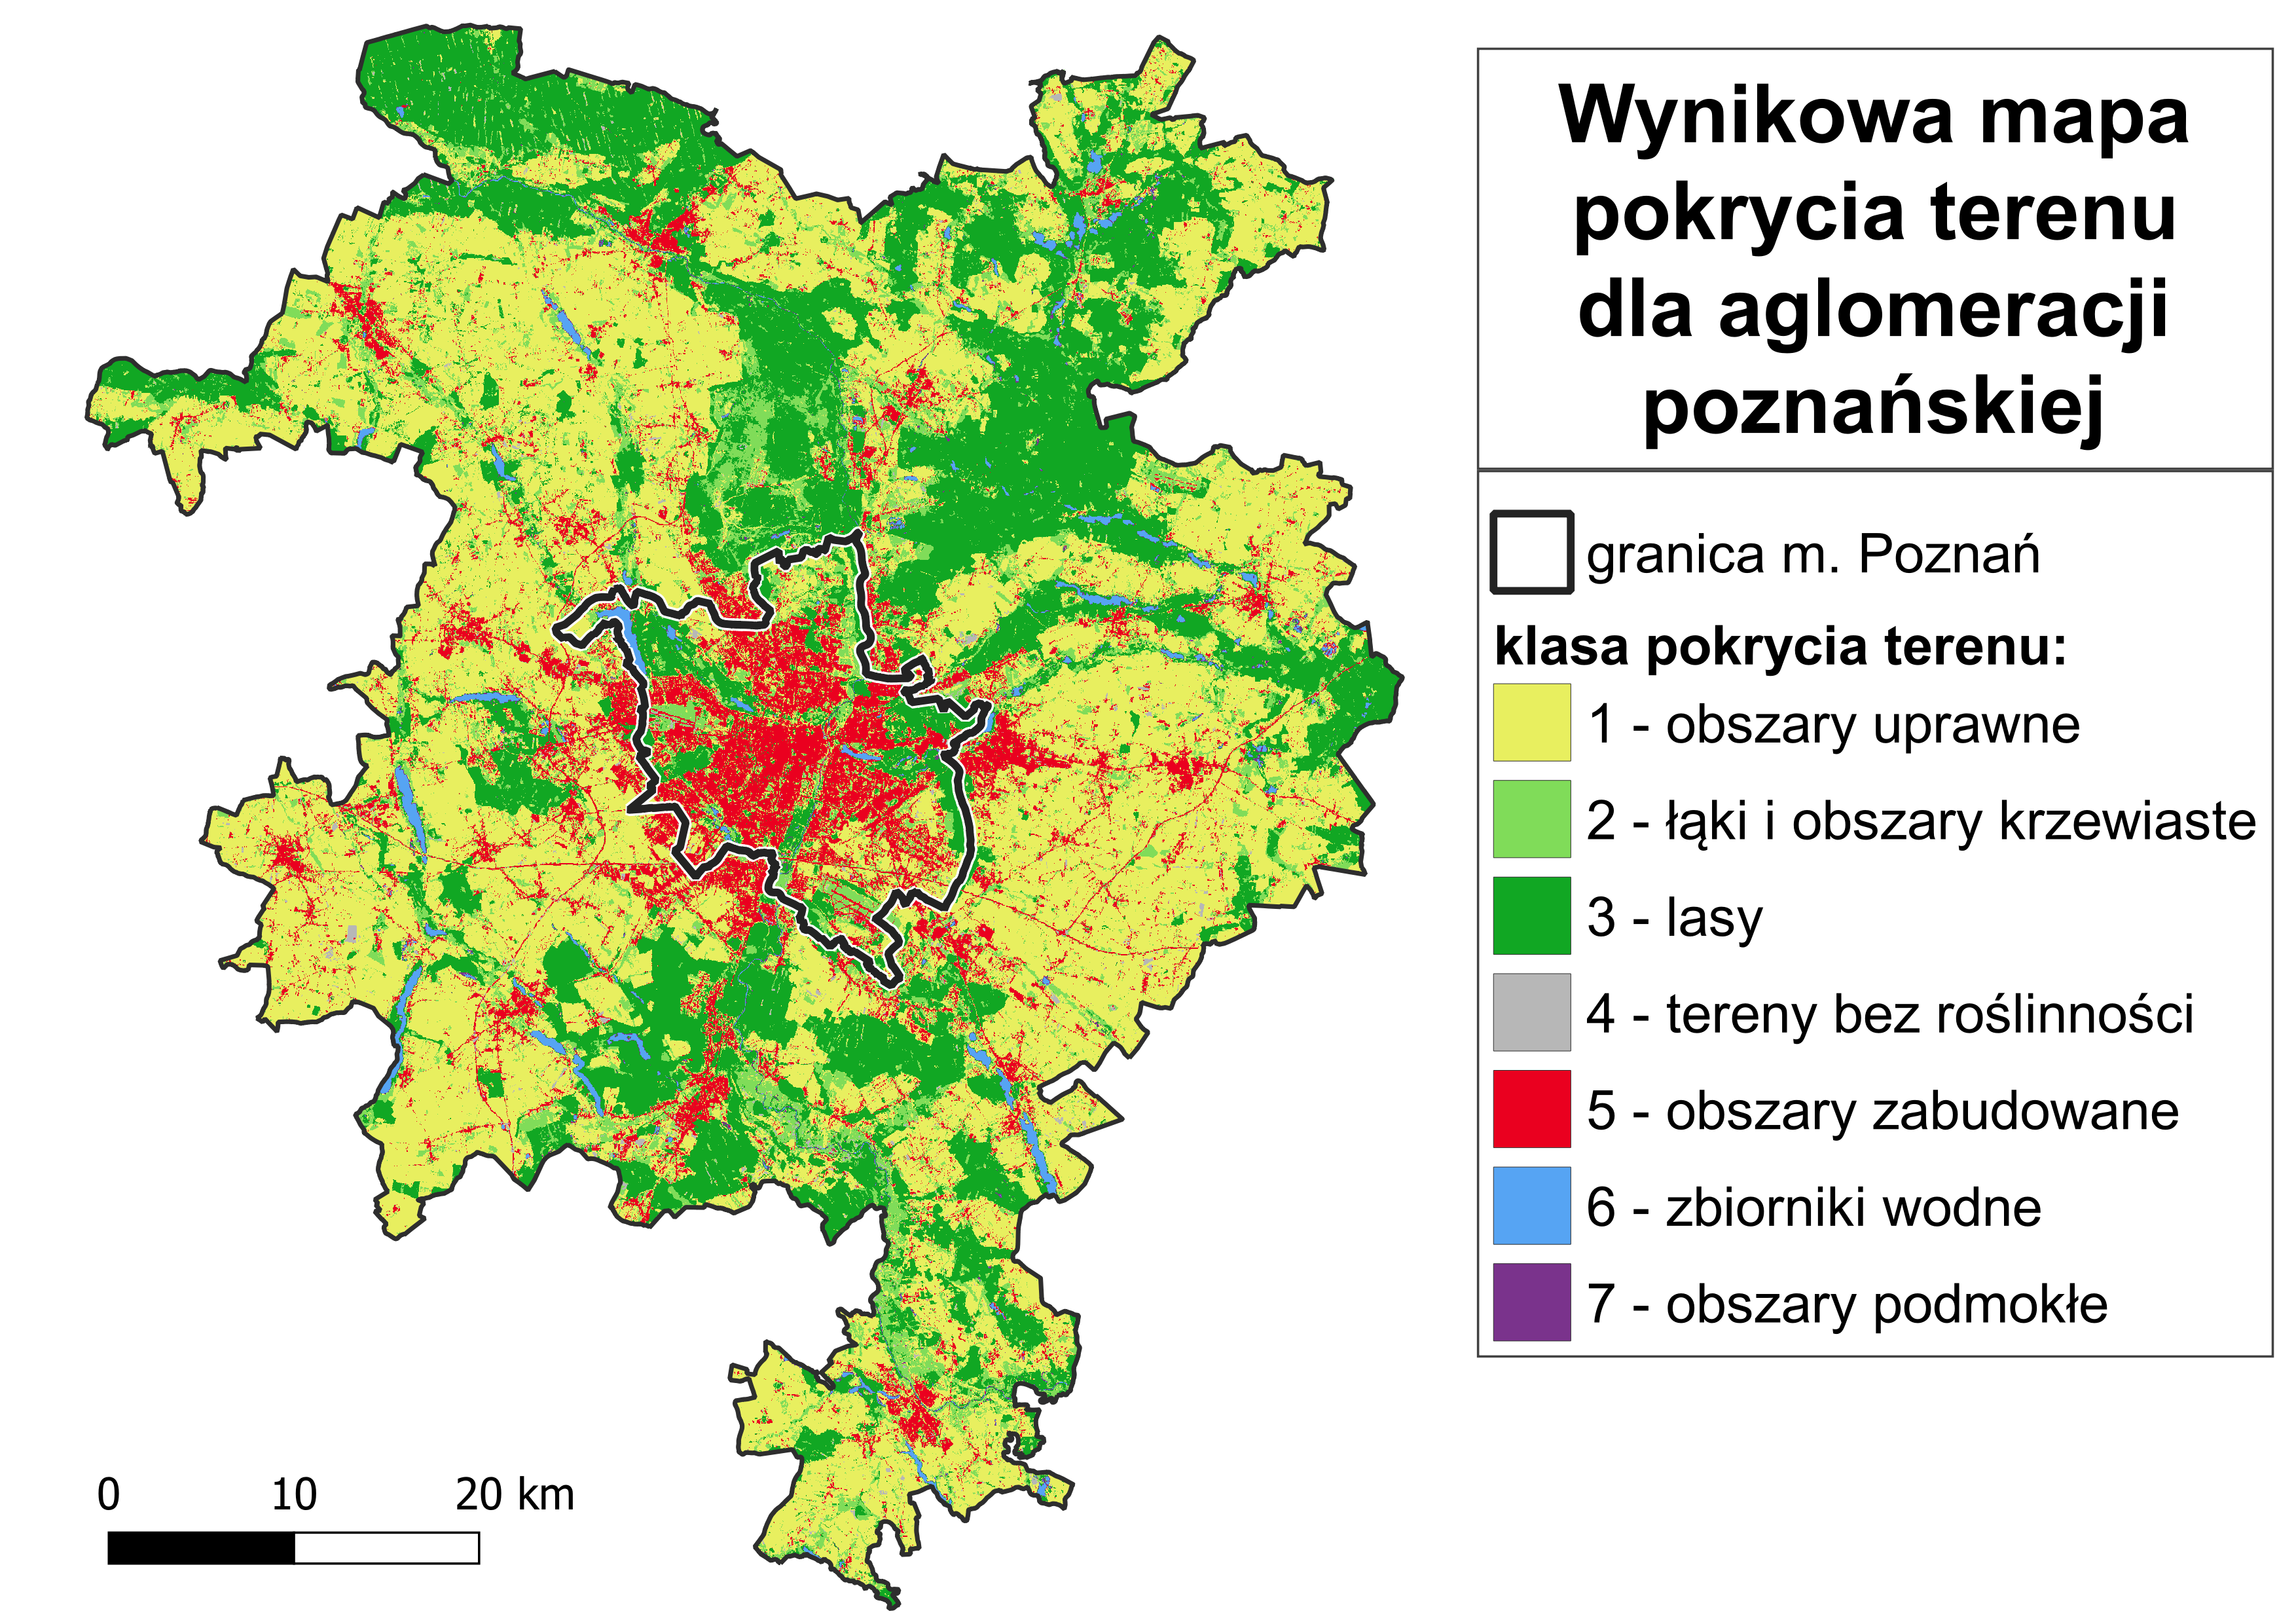
\includegraphics[width=5.875in,height=4.16667in]{./figures/result_map.png}

}

\caption{\label{fig-rycina10}Comparison of created land cover map with
RGB imagery.}

\end{figure}

\begin{itemize}
\tightlist
\item
  probability map of model results
\end{itemize}

\begin{figure}[t]

{\centering 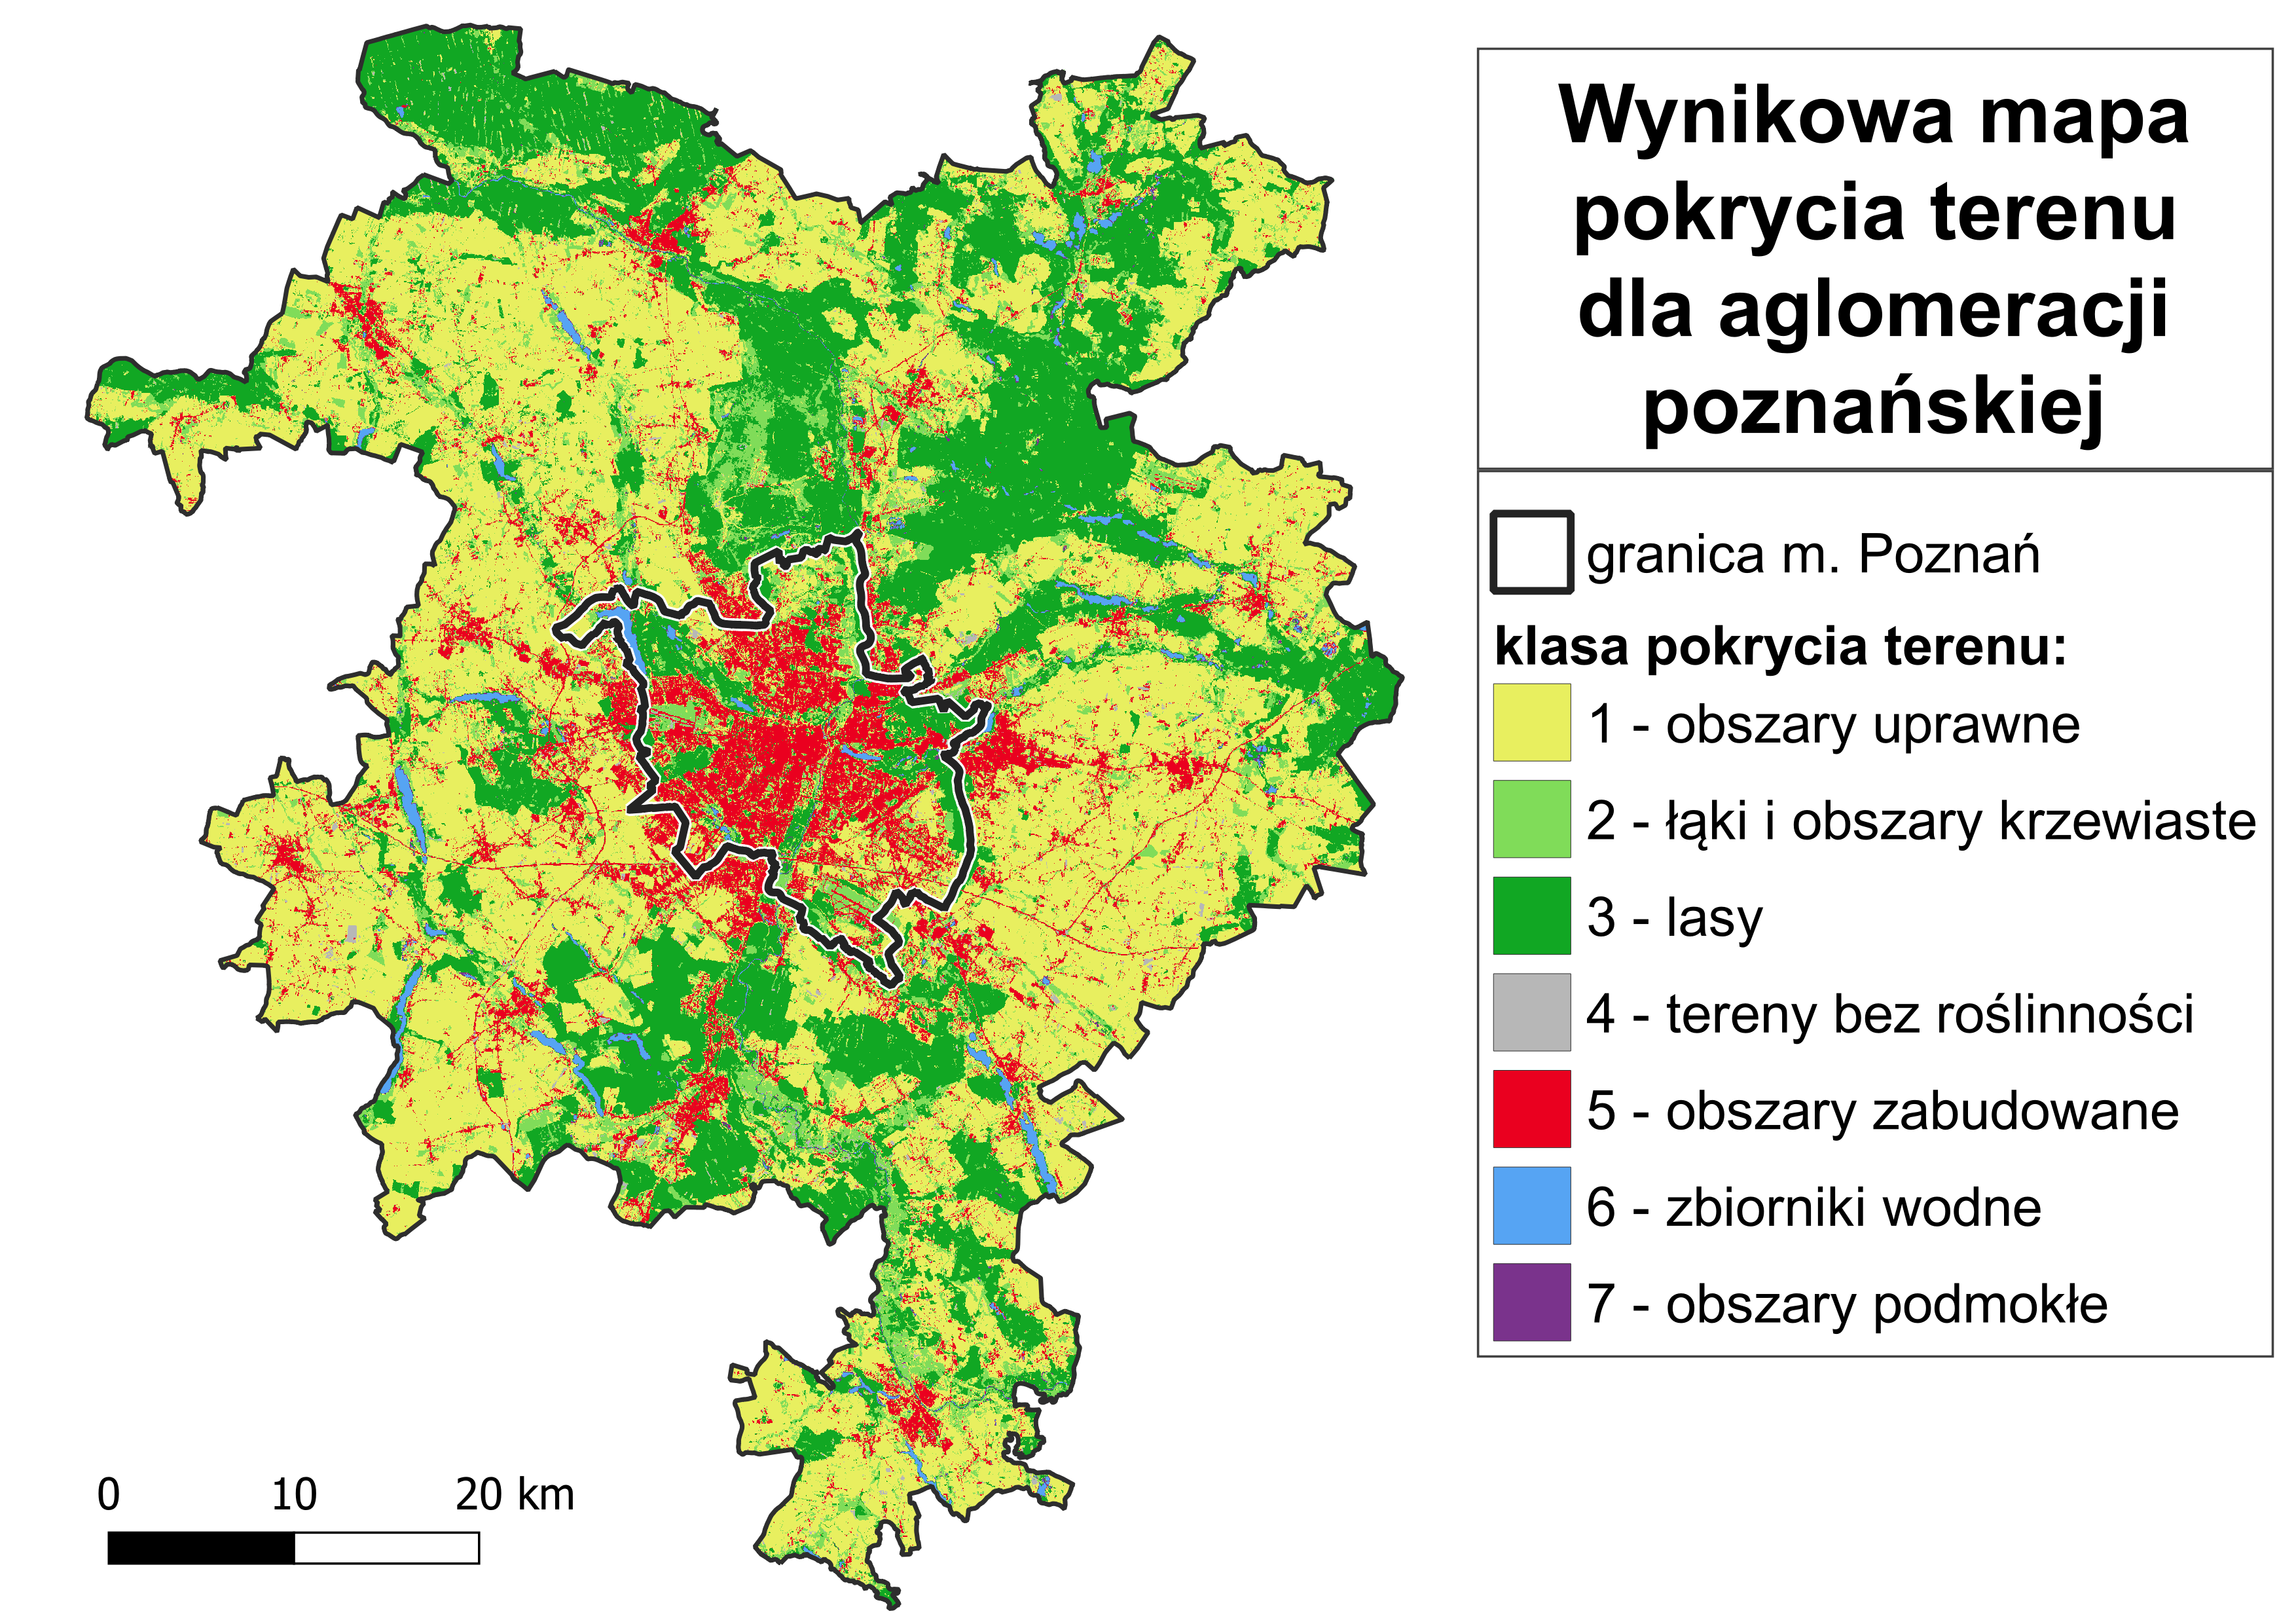
\includegraphics[width=5.875in,height=4.16667in]{./figures/result_map.png}

}

\caption{\label{fig-rycina11}Probability of chosen land cover class
being present on the ground. This can be treated as confidence of model
on its results.}

\end{figure}

\bookmarksetup{startatroot}

\hypertarget{sec-results-eval}{%
\chapter{Assessing model quality}\label{sec-results-eval}}

Table with quality indices:

\begin{itemize}
\item
  overall accuracy (OA) / classification error (CE)
\item
  producer's and user's accuracy (PA, UA) / precission and recall
\item
  F1-score
\item
  Kappa coefficient
\end{itemize}

\hypertarget{tbl-tabela4}{}
\begin{table}
\caption{\label{tbl-tabela4}Measures of overall model accuracy calculated during
cross-validation/resampling process. }\tabularnewline

\centering
\begin{tabular}{|>{}l|>{}r|}
\toprule
\textbf{Measure} & \textbf{Avg. value}\\
\midrule
overall accuracy & 0.75\\
\hline
Kappa coefficient & 0.70\\
\hline
precission & 0.80\\
\hline
recall & 0.78\\
\hline
F1-score & 0.79\\
\bottomrule
\end{tabular}
\end{table}

\hypertarget{tbl-tabela5}{}
\begin{table}
\caption{\label{tbl-tabela5}Accuracy measures by land cover class. }\tabularnewline

\centering
\begin{tabular}{|>{}l|>{}r|>{}r|>{}r|}
\toprule
\textbf{Land cover class} & \textbf{Precision (producer's accuracy)} & \textbf{Recall (user's accuracy)} & \textbf{F1-score}\\
\midrule
arable land & 0.8 & 0.75 & 0.8\\
\hline
grasslands & 0.8 & 0.70 & 0.8\\
\hline
forests & 0.8 & 0.80 & 0.8\\
\hline
bare land & 0.8 & 0.78 & 0.8\\
\hline
artificial land & 0.8 & 0.79 & 0.8\\
\hline
water bodies & 0.8 & 0.80 & 0.8\\
\hline
wetlands & 0.8 & 0.80 & 0.8\\
\bottomrule
\end{tabular}
\end{table}

\bookmarksetup{startatroot}

\hypertarget{sec-results-therm}{%
\chapter{Evaluation of thermal band's impact on prediction
results}\label{sec-results-therm}}

\hypertarget{sec-imp-overall}{%
\section{Overall importance of thermal band}\label{sec-imp-overall}}

\begin{itemize}
\item
  mean temperature for every predicted land cover class
\item
  mean importance of thermal band on each land cover class
\end{itemize}

\hypertarget{tbl-tabela6}{}
\begin{table}
\caption{\label{tbl-tabela6}Mean value and importance of thermal band, by land cover class. }\tabularnewline

\centering
\begin{tabular}{|>{}l|>{}r|>{}r|}
\toprule
\textbf{Land cover class} & \textbf{Avg. value} & \textbf{Avg. importance}\\
\midrule
arable land & 0.8 & 0.75\\
\hline
grasslands & 0.8 & 0.70\\
\hline
forests & 0.8 & 0.80\\
\hline
bare land & 0.8 & 0.78\\
\hline
artificial land & 0.8 & 0.79\\
\hline
water bodies & 0.8 & 0.80\\
\hline
wetlands & 0.8 & 0.80\\
\bottomrule
\end{tabular}
\end{table}

\begin{itemize}
\tightlist
\item
  variable importance plots, variable profiles
\end{itemize}

\begin{figure}[t]

{\centering 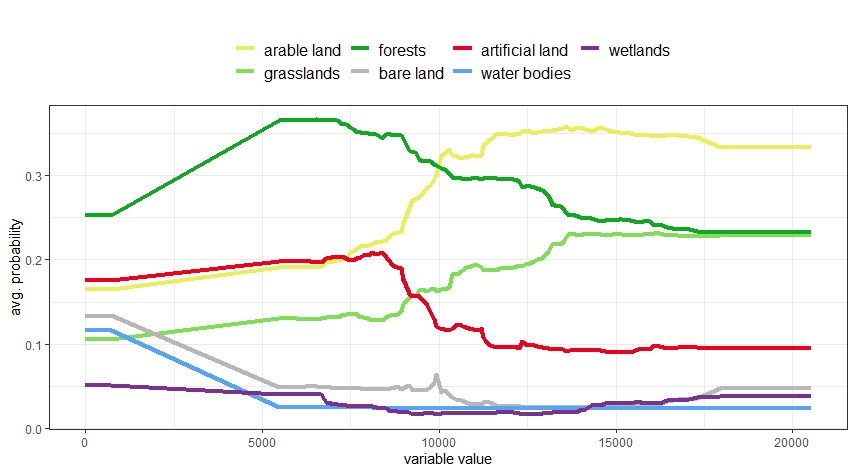
\includegraphics[width=5.90625in,height=3.125in]{./figures/profB5.png}

}

\caption{\label{fig-rycina12}Variable profile for near-infrared band
(B5).}

\end{figure}

\begin{figure}[t]

{\centering 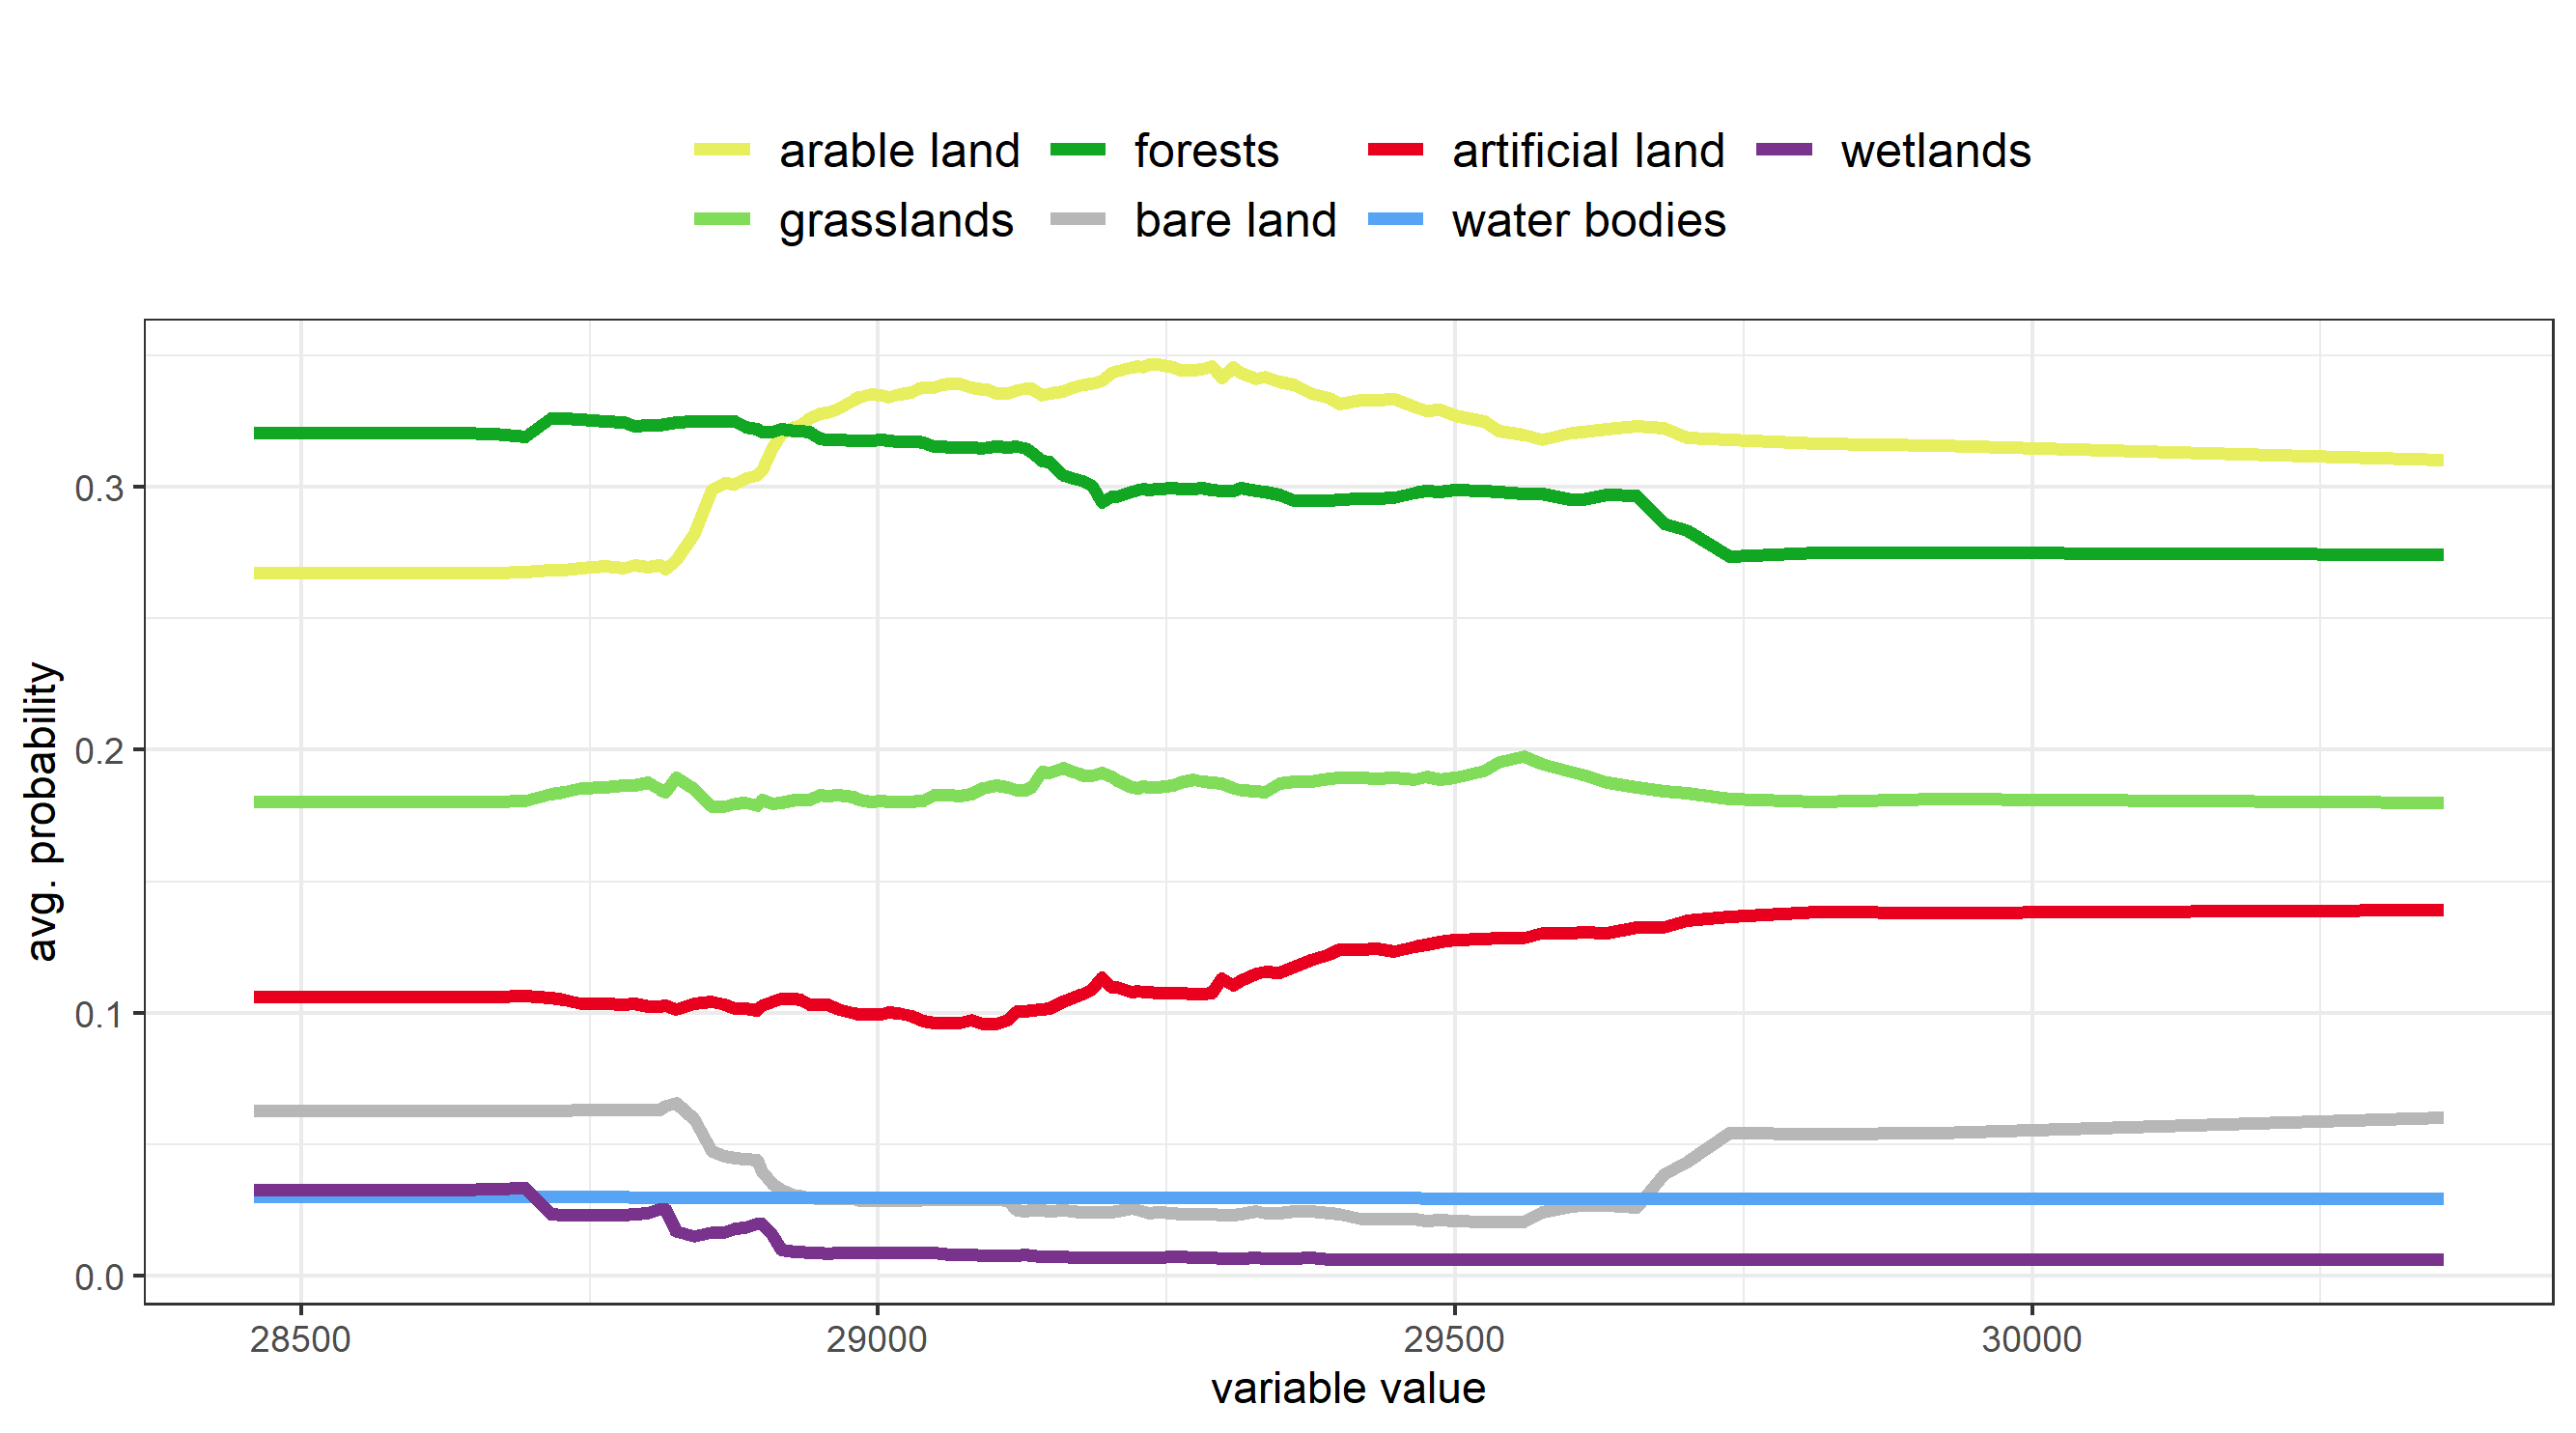
\includegraphics[width=5.90625in,height=3.125in]{./figures/profB10.png}

}

\caption{\label{fig-rycina13}Variable profile for thermal band (B10)}

\end{figure}

\hypertarget{sec-imp-spat}{%
\section{Spatial distribution of thermal band's
importance}\label{sec-imp-spat}}

\begin{itemize}
\tightlist
\item
  thermal band importance map (two methods: raster aggregation and
  interpolation of importance in LUCAS points)
\end{itemize}

\begin{figure}[t]

{\centering 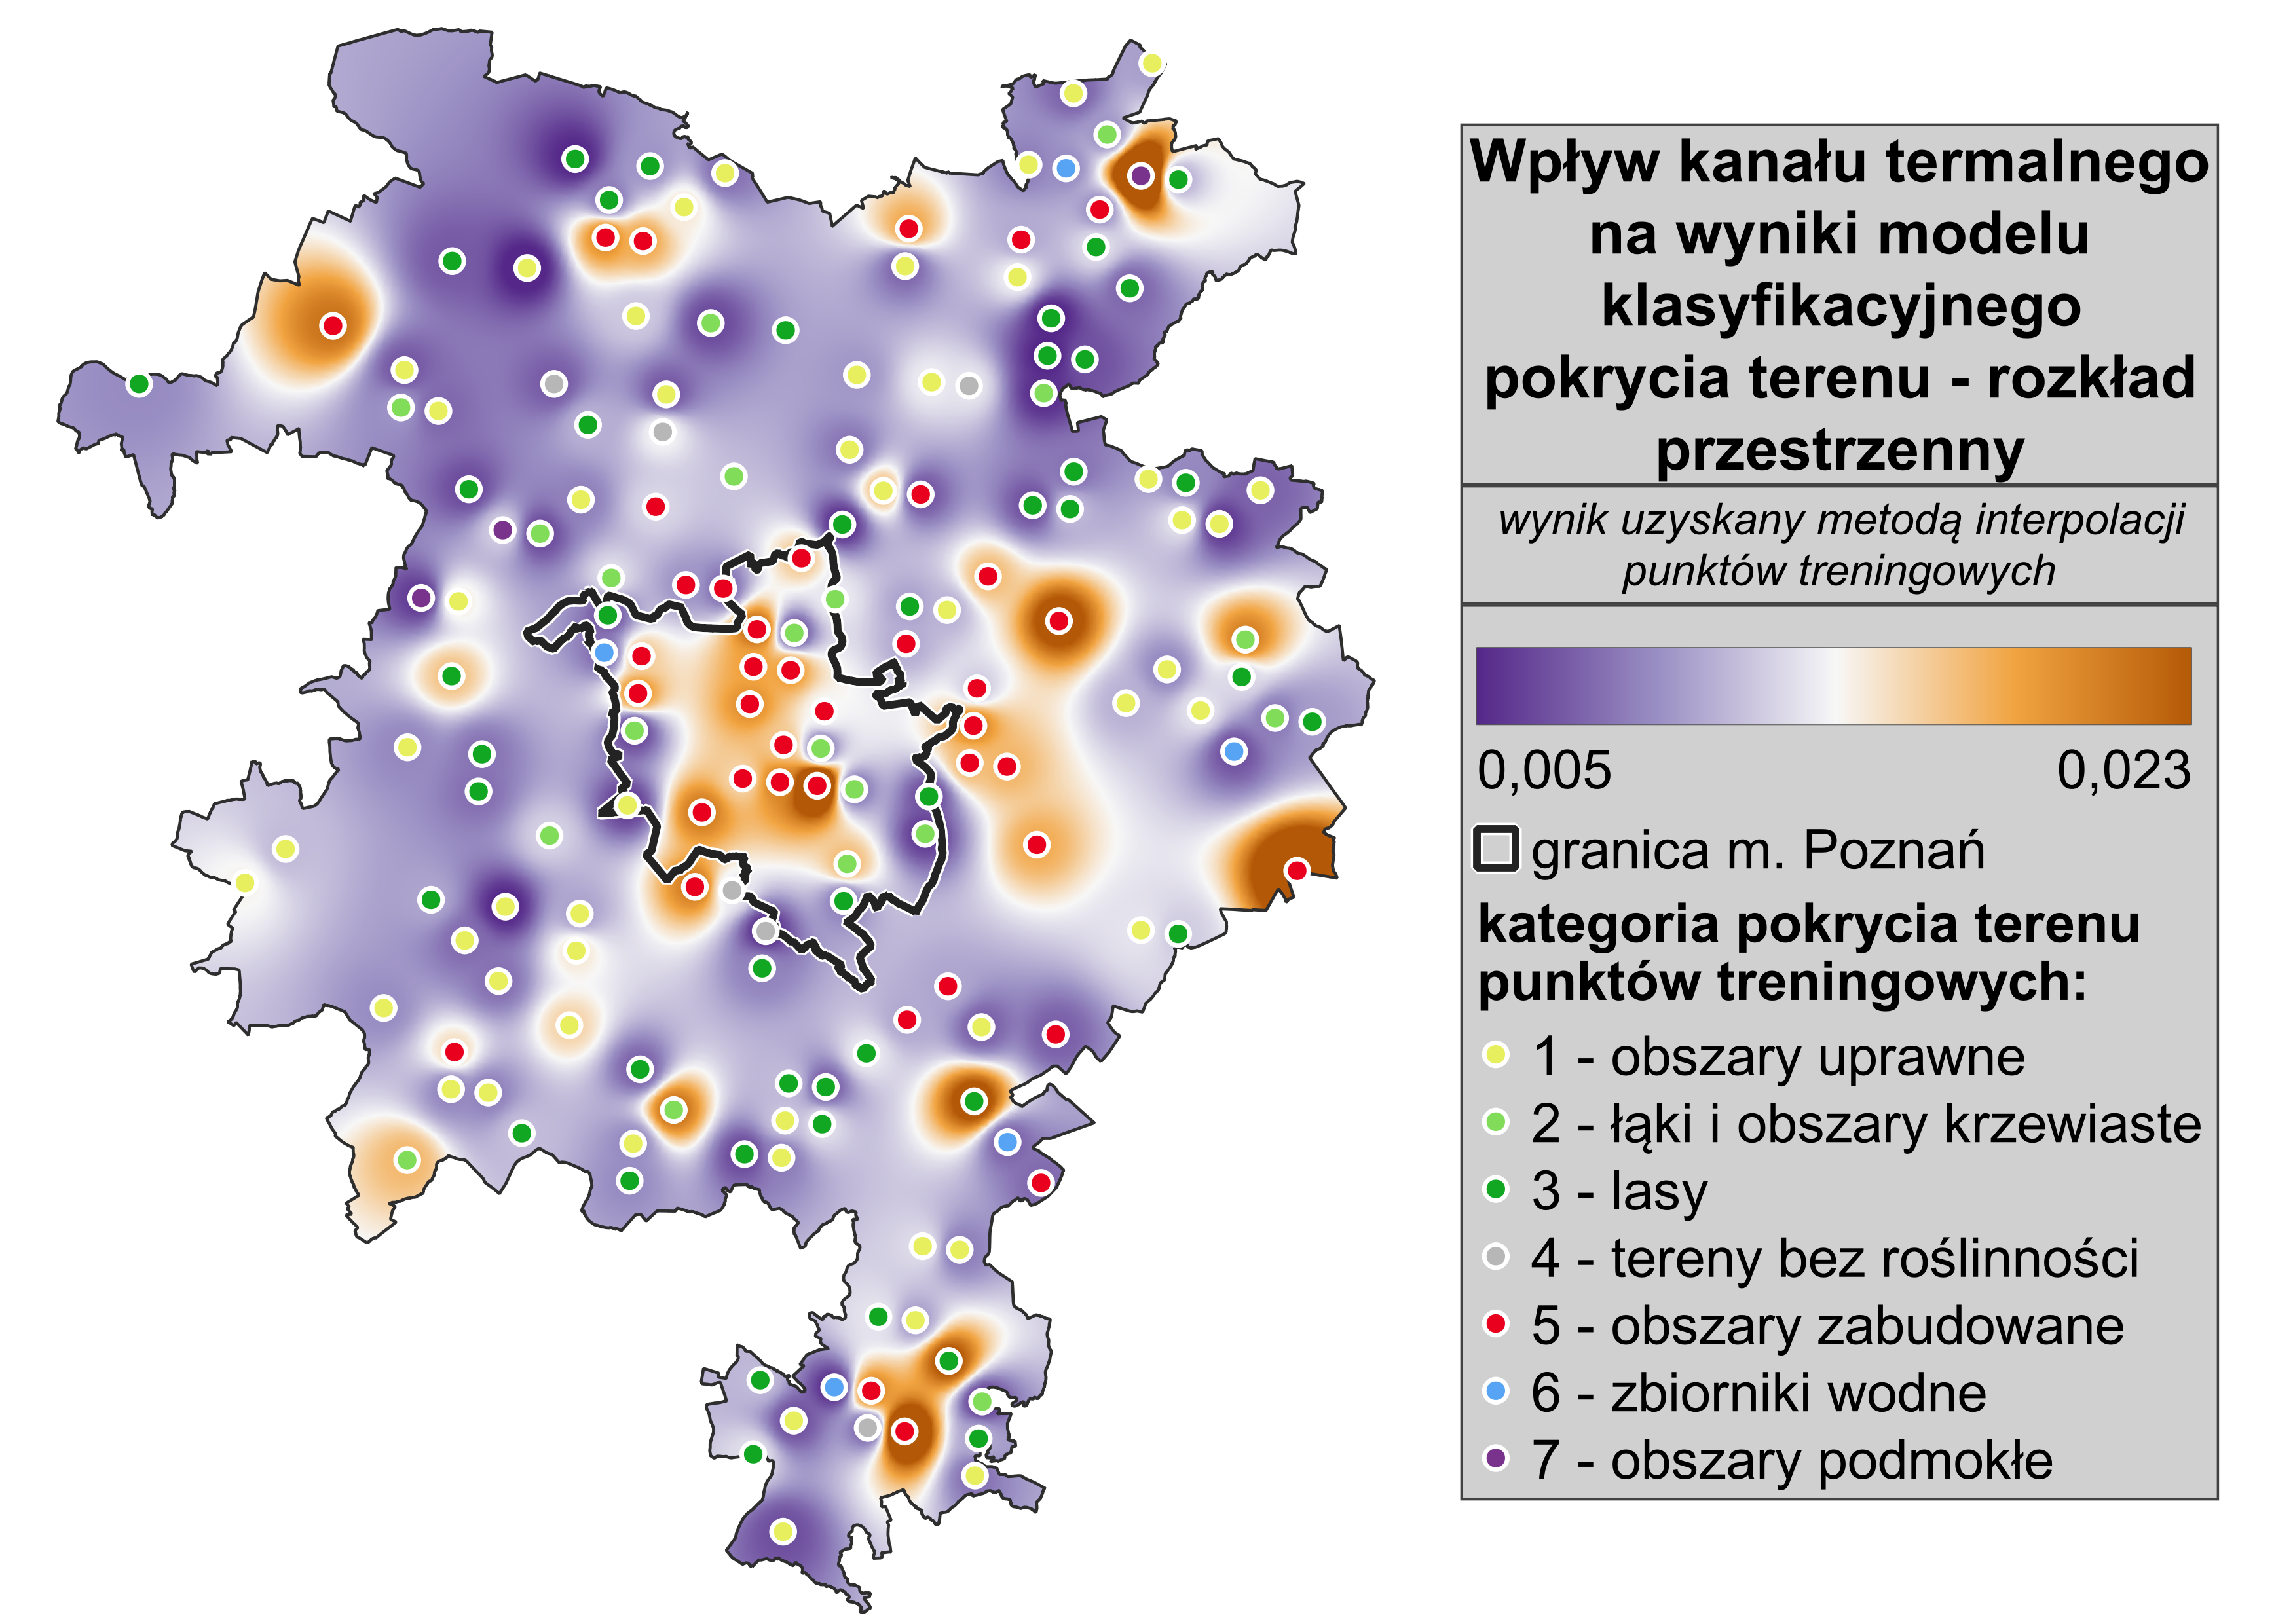
\includegraphics[width=5.875in,height=4.16667in]{./figures/B10_importance-spatial.png}

}

\caption{\label{fig-rycina14}Thermal band importance calculated for
raster cells aggregated to 1,5 km resolution.}

\end{figure}

\begin{figure}[t]

{\centering 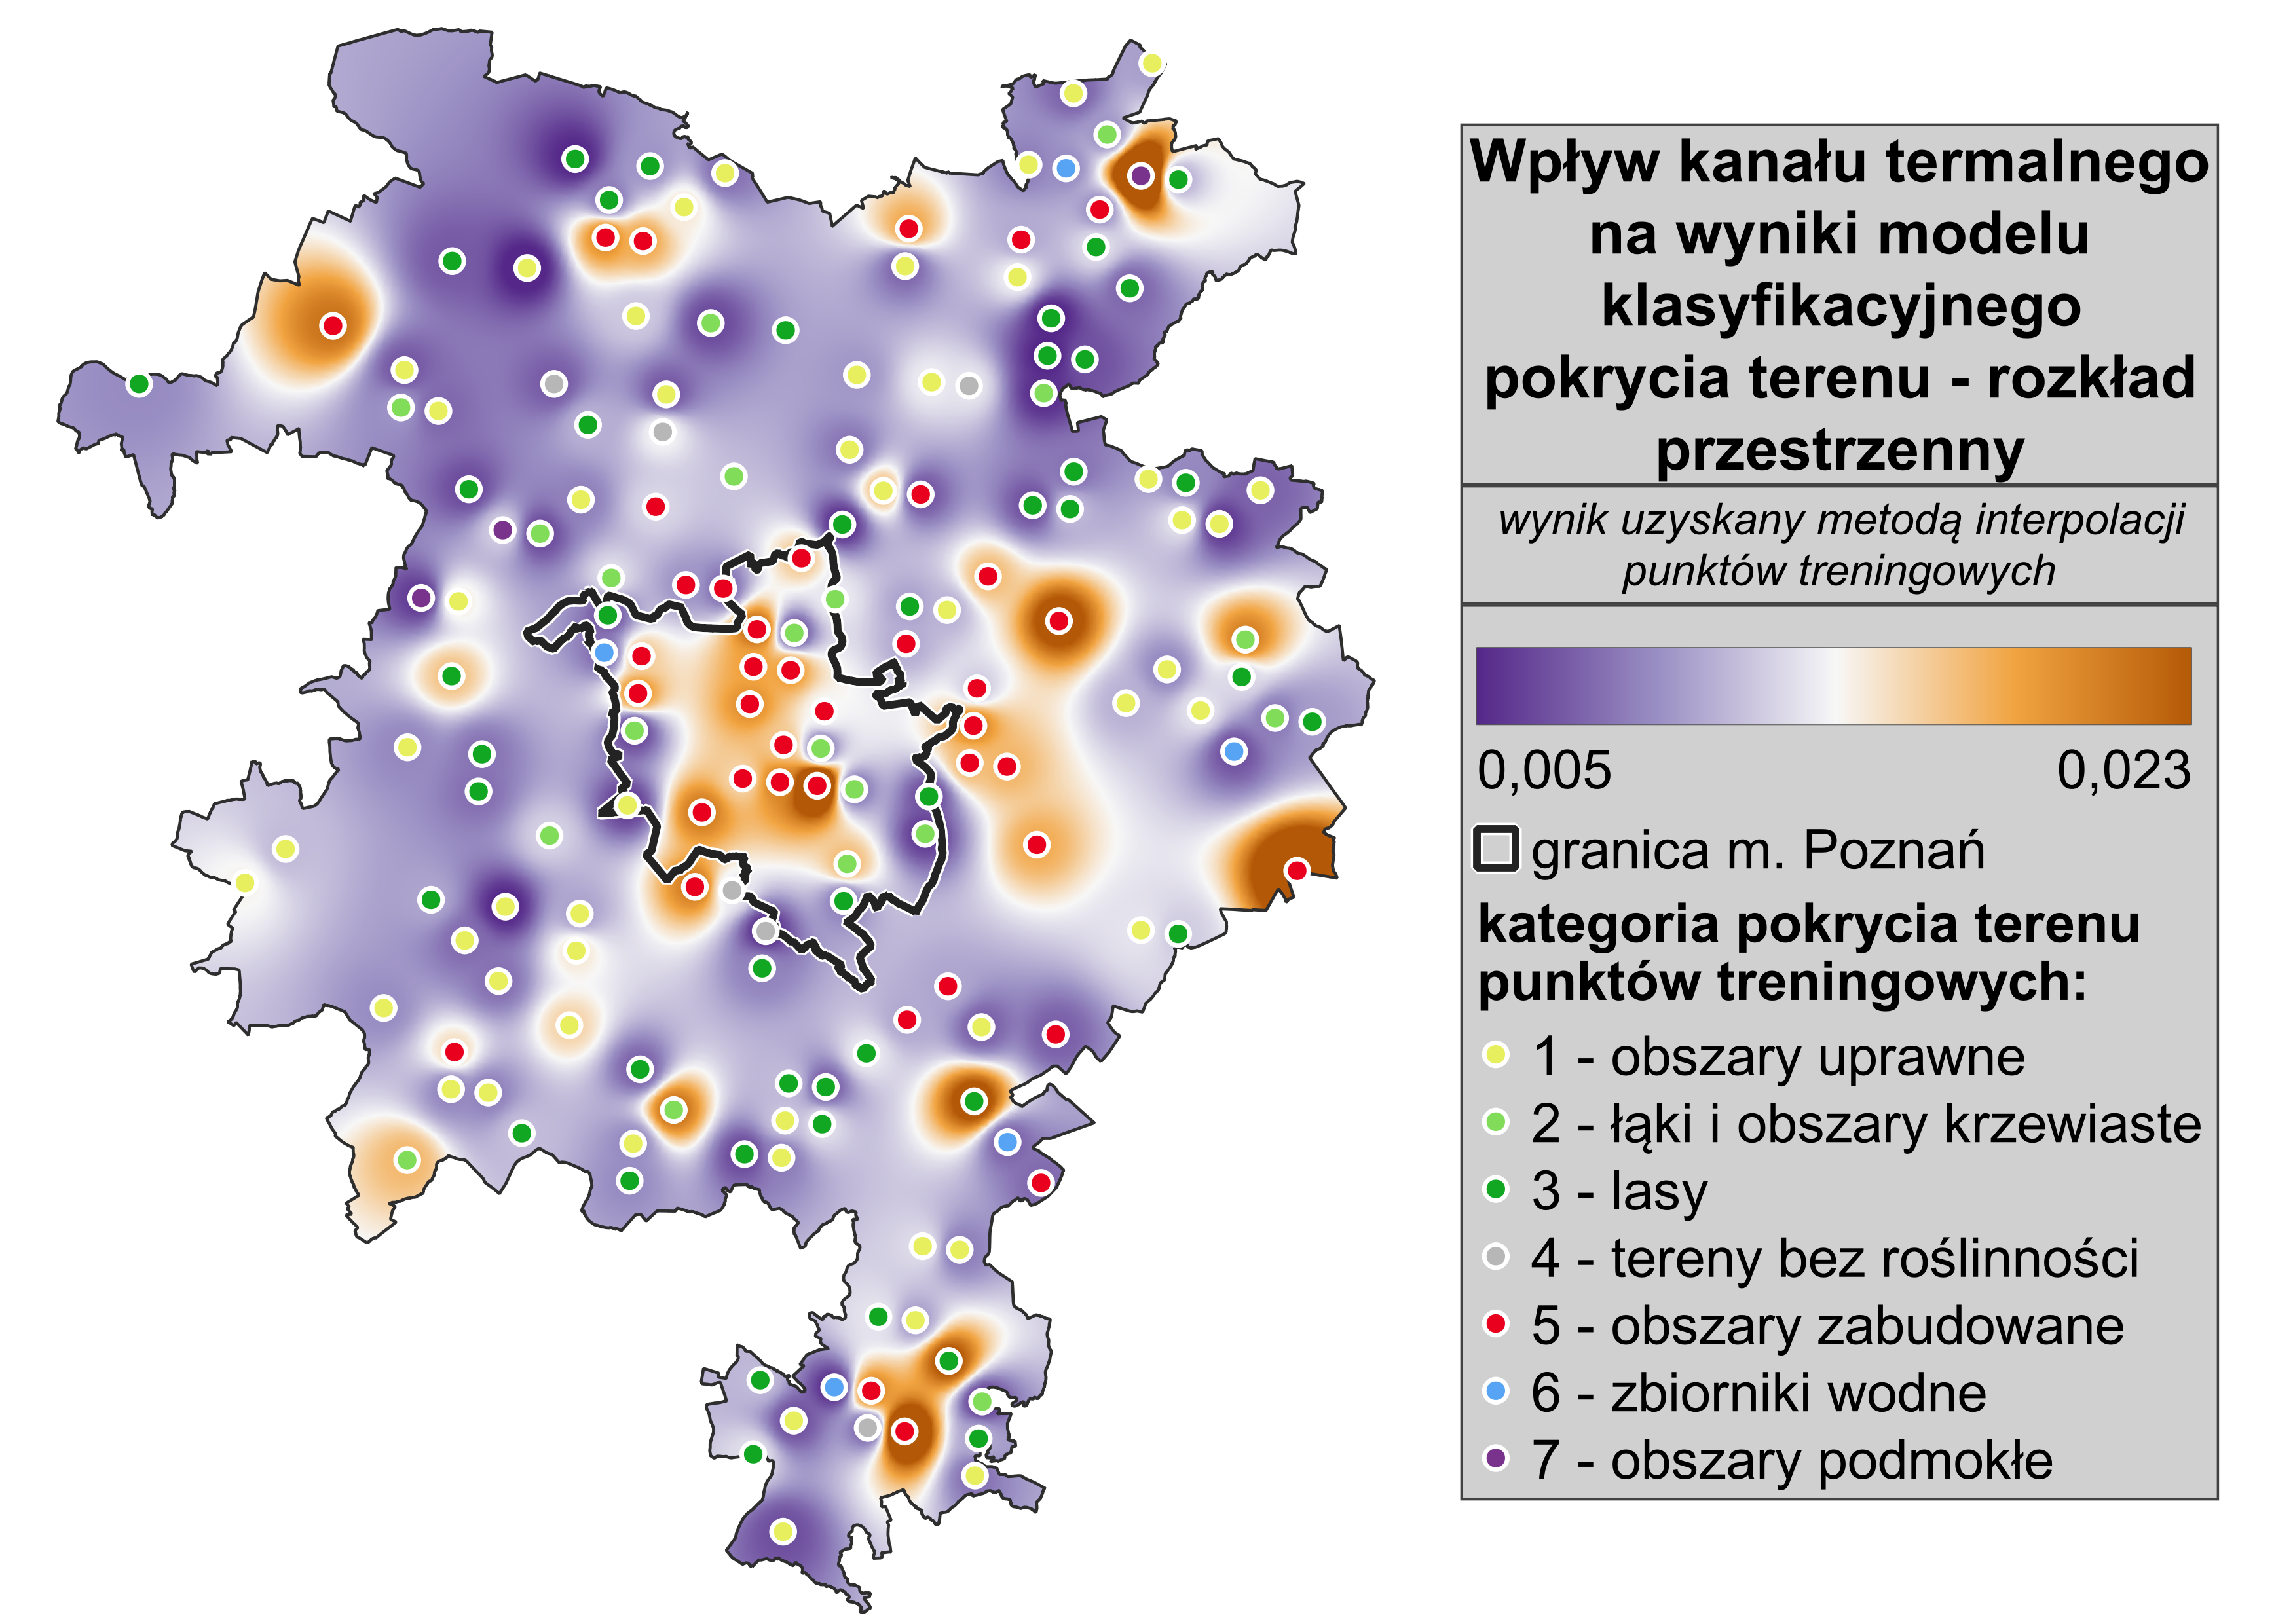
\includegraphics[width=5.875in,height=4.16667in]{./figures/B10_importance-spatial.png}

}

\caption{\label{fig-rycina15}Thermal band importance interpolated from
values on LUCAS points locations.}

\end{figure}

\begin{itemize}
\tightlist
\item
  difference raster map between prediction with and without thermal band
  included, transition matrix (?)
\end{itemize}

\bookmarksetup{startatroot}

\hypertarget{conclusion}{%
\chapter{Conclusion}\label{conclusion}}

\begin{itemize}
\item
  land cover map of Poznań metropolitan area was created, impact of
  thermal band on classification results was measured
\item
  despite thermal band having low overall impact on model results, there
  is a strong spatial auto-correlation for its importance
\item
  land surface temperature was especially significant for land cover
  classification of urban areas, it helped in identify built-up areas
\item
  it may mean that thermal band will become increasingly important in
  studies on urban sprawl and suburbanisation
\item
  better land cover maps will help in better management of metropolitan
  areas growth and quantifying impact of urbanisation on natural
  environment more precisely
\end{itemize}

\begin{center}\rule{0.5\linewidth}{0.5pt}\end{center}

Podsumowanie pracy jest w pewnym sensie znacznie rozbudowanym
abstraktem. Należy wyliczyć i opisać osiągnięcia uzyskane w pracy
dyplomowej. Tutaj jednak (w przeciwieństwie do np. rozdziału
\textbf{?@sec-wprowadzenie}) należy przechodzić od szczegółu do ogółu -
co zostało stworzone/określone, jak zostało to zrobione, jakie ma to
konsekwencje, itd.

Ten rozdział powinien też zawierać opis kwestii, których nie udało się
rozwiązać w pracy dyplomowej (i dlaczego się nie udało) oraz pomysły na
przyszłe ulepszenie uzyskanych wyników lub dalsze badania.

\printbibliography[heading=bibintoc, title=Bibliography]

\end{document}
